
\section{Open questions from PSTN-055} \label{sec:openquestions}

\subsection{Swapping filters on the filter wheel}\label{sec:filterswap}
The filter system at Rubin allows five of the six filters to be mounted at the same time on the carousel. Filters at the edge of the system transmission will be swapped in and out of the filter wheel throughout the lunar cycle. In \citetalias{PSTN-055} Section 4 the SCOC recommended further investigation of which filters to swap: 
\begin{quote}{[\citetalias{PSTN-055}] ``The SCOC recommends that the investigation of the filter swapping schemes on the filter wheel continue. After the November 2022 SCOC workshop, a few experiments in swapping $u$, $z$, and $y$ instead of $u$ and $z$ were implemented in \texttt{v2.99} simulations. More work is needed to understand the impacts of this decision on the DDFs as well as on the WFD. Filter pairing prescriptions for the observation pairs should also be explored in some more depth.''}
\end{quote}

 Simulations prior to \texttt{v3.0} swapped the $z$ with $u$ based on lunation, as moonlight is blue and impacts observations in $u$-band most significantly. Simulations tagged \texttt{v3.2}  experimented with  swapping $u$ with $z$ or $y$, including putting all of $u$, $z$, and $y$ on rotation. Increasing the availability of $z$ on the filter wheel produced significant improvements in supernova (SN) cosmology, especially in the Deep Drilling Fields (DDFs), while swapping two filters, instead of three, improves coverage at short time scales in filters through $z$ (see \autoref{fig:swapping}). 
 
{\it The SCOC recommends swapping $u$- and $y$-band according to the moon phase. This produces benefits for SN cosmology while preserving coverage on short timescales. This recommendation is implemented starting in \baseline{3.2}}.

\begin{figure}
\centering
%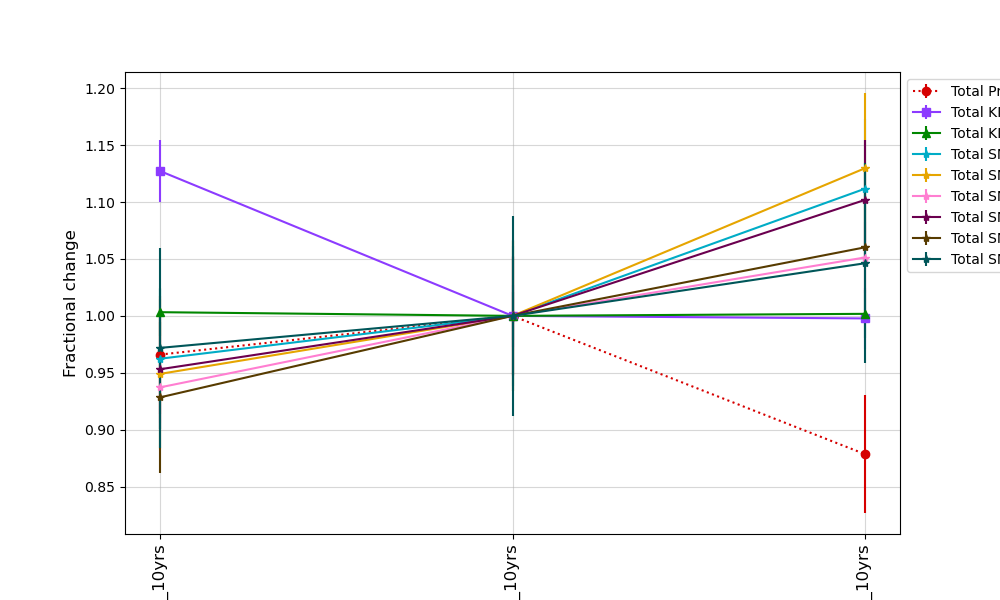
\includegraphics[width=0.5\textwidth]{figures/filter_swap_linear.png}
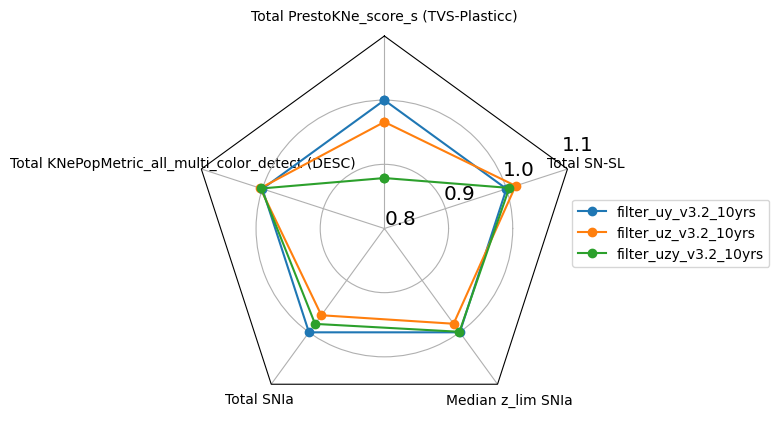
\includegraphics[width=0.45\textwidth]{figures/filter_swap_KNe.png}
%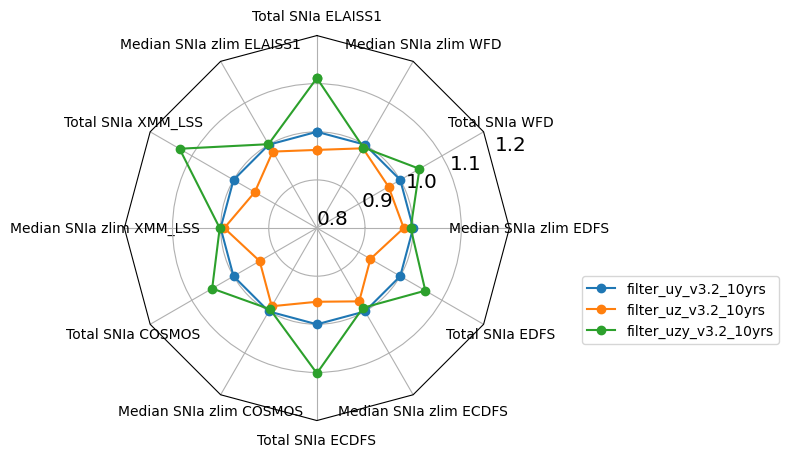
\includegraphics[width=0.45\textwidth]{figures/filter_swap_SNIa.png}
\caption{Swapping a filter out of the camera has two effects: it adds a gap for the period of time while it's unavailable, and it increases the cadence in that bandpass during the time it is in the camera. Gaps in $z$ band are particularly bad for SNIa detections, an effect which is magnified for Deep Drilling Fields. %Increases in $z$ band cadence can be beneficial for KNe detection, if repeated observations in the same filter within a rapid timeframe is the criteria. 
Swapping three filters ($u$ with alternating $z$ and $y$) increases the length of time gaps between sampling in the same filter, decreasing performance for hours-days transients.
Swapping $u$ with $y$ while leaving $z$ mounted on the filter wheel has an overall positive science impact, balancing the impact to a variety of needs for rapid transient science with SNIa science in the Deep Drilling Fields. }
\label{fig:swapping}
\end{figure}

\FloatBarrier
\subsection{Filter Balance}\label{sec:filterbalance}
 In \citetalias{PSTN-055}, the SCOC confirmed the recommendation on the filter balance as implemented starting in \baseline{2.0} but left the possibility that:
  
 \begin{quote}[\citetalias{PSTN-055}] ``While the SCOC recommends the filter balance as implemented starting in \texttt{baseline\v2.0} should not be changed, it is possible that rebalancing the
exposure time to compensate for performance and throughput in some filters as compared to others or shortening exposures in filters where the throughput exceeds expectations enabling the collection of more images in that filter (or overall) would lead to
enhanced LSST science. The SCOC cannot finalize this recommendation at this time due to
missing information about the characteristics of the system-as-built.''
\end{quote}

Simulations of the survey strategy up to and including \baseline{3.2} use throughput curves assuming mirror coating as Al-Ag-Al respectively for M1-M2-M3. Conversely, the plan to coat the mirrors was updated in 2023 to Ag-Ag-Ag (or 3xAg), which leads to a $\sim15-20\%$ increase in survey efficiency compared to Al-Ag-Al by increasing throughput in all bands redder than $u$, and bringing throughput closer to the design goals as stated in \citetalias{LPM-17}.\footnote{\url{https://community.lsst.org/t/rubin-sim-v1-3-released/7937} and \url{https://github.com/lsst-pst/syseng_throughputs/blob/main/notebooks/SilverVsAluminum.ipynb}.}  \autoref{tab:dm5Agx3} shows the magnitude limit changes associated with coating.  3xAg coating increases sensitivity in all LSST bands from $g$ to $y$, but it decreases the throughput in $u$.  As of \baseline{3.3}, all \opsim\ simulations include the updated expected throughput.

\begin{longtable}{lcccc}
 \\\hline
& Al-Ag-Al E2V &	Al-Ag-Al ITL &		Ag-Ag-Ag E2V &		Ag-Ag-Ag ITL\\
\hline
$u$	 &	0.0	 &	-0.06 &		-0.21 &		-0.27\\
$g$	 &	0.0	 &	-0.04 &		0.06 &		0.02\\
$r$	 &	0.0	 &	-0.05 &	    0.10 &	 0.05\\
$i$	 &	0.0	 &	-0.02 &		0.13 &		0.12\\
$z$	 &	0.0	 &	0.01  &		0.15  &		0.15\\
$y$	 &	0.0	 &	0.03  &		0.07  &		0.10\\
\caption{Magnitude limit change, compared to expected magnitude limit with E2V chips coated with Al-Ag-Al. Note: values are reported for chips acquired by two different filter vendors as E2V and ITL for both coating schemes. Positive values indicate deeper limiting magnitudes.
}\label{tab:dm5Agx3}
\end{longtable}
The SCOC reviewed the largely positive impact of the new throughput on science cases: nearly all MAFs responded positively to the increase in survey depth with some metrics showing improvements as large as 10\% (\eg\ Parallax uncertainty, see \autoref{fig:parallax}, see also \autoref{fig:heatmap} and note the significant improvements between \baseline{3.2} and \baseline{3.3} when the new filter transmission curves were introduced). 

\begin{figure}
    \centering

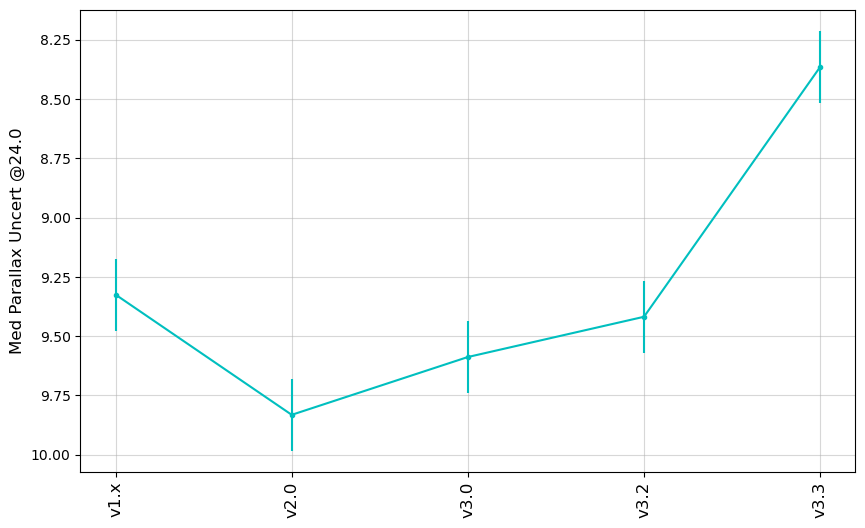
\includegraphics[width=0.8\textwidth]{figures/baseline_parallax.png}
\caption{Gains in the metric tracking LSST's median Proper motion at magnitude $r=24$, a standard metric that measures a LSST \citetalias{LPM-17} system requirement for different $\mathrm{baseline}$ \opsim s, from \baseline{1.x} through \baseline{3.0}, and additional \opsim s  through $v3.3$: the first simulation with updated system throughput. The improvements in parallax uncertainty between $v3.2$ and $v3.3$ \opsim\ come from the change in throughput and added depth in all bands bluer than $u$. }
\label{fig:parallax}
\end{figure}

However, the SCOC understands that the throughput loss in $u$-band ($\sim30\%$  loss in coadded depth) would negatively impact science cases including Photo-z, studies of the Milky Way halo, Lyman Break Galaxies (LBGs, identified as $u$-band dropouts at redshift $z\sim3$), and more. While the overwhelming majority of the MAF metrics available to the SCOC responded positively to the updated throughput, we are aware, as always, that these may not provide an exhaustive picture of the science outcomes. Therefore, guided by experts in the community, we explored ways to reduce the $u$ band magnitude decrease while preserving the benefit of increased throughput in redder bands. 
We tracked the performance of Photo-z, as characterized in \citealt{Graham_2017}, by assessing the variance and bias in \pz\ at redshifts $z\lesssim{3}$. \pz\ is sensitive to $u$ band depth at redshift $z\geq 2$ due to decrease power to identify Lyman break galaxies photometrically. We expect that recovering \pz\ performance is a good indicator of recovering performance for other science cases sensitive to $u$ band depth for which we do not have detailed metrics. \pz\ performance, along with a large set of MAFs, were run against a set of \opsim s  that progressively changed the exposure time and the number of exposures in $u$-band\footnote{\url{https://community.lsst.org/t/release-of-v3-4-simulations/8548}}. 

\emph{The SCOC recommends:} 

\begin{itemize} 
\item \emph{an increase of the exposure time in $u$-band to 38 seconds per visit}
\item \emph{an increase of the number of $u$-band visits of 10\% compared to \baseline{3.0}}
\item \emph{an identical decrease of 0.8 second exposure time in all other bands to compensate for the added time in $u$-band.} 
\end{itemize}


This roughly restores the $u$ band depth of LSST in \baseline{3.0} with minimal impact on LSST science metrics. As a science case that is representative of those sensitive to $u$-band depth, these changes recover performance on \pz\ at redshift $z\sim2$, where the impact of the $u$-band throughput loss was most significant while maintaining the performance improvement on \pz\ at low redshift afforded by the increased depth of LSST in all other bands. Furthermore, these changes minimally impact other science cases tracked by MAFs. 

Since more science cases generally respond better to increasing the number of images, over increasing the exposure time to achieve the same depth, the added $u$-band time should be obtained by decreasing (minimally) the exposure time in other bands, rather than decreasing the number of images.

\textbf{ We note that this recommendation is subject to ongoing feasibility studies by the Rubin Data 
Management team.}

\begin{figure}
\centering
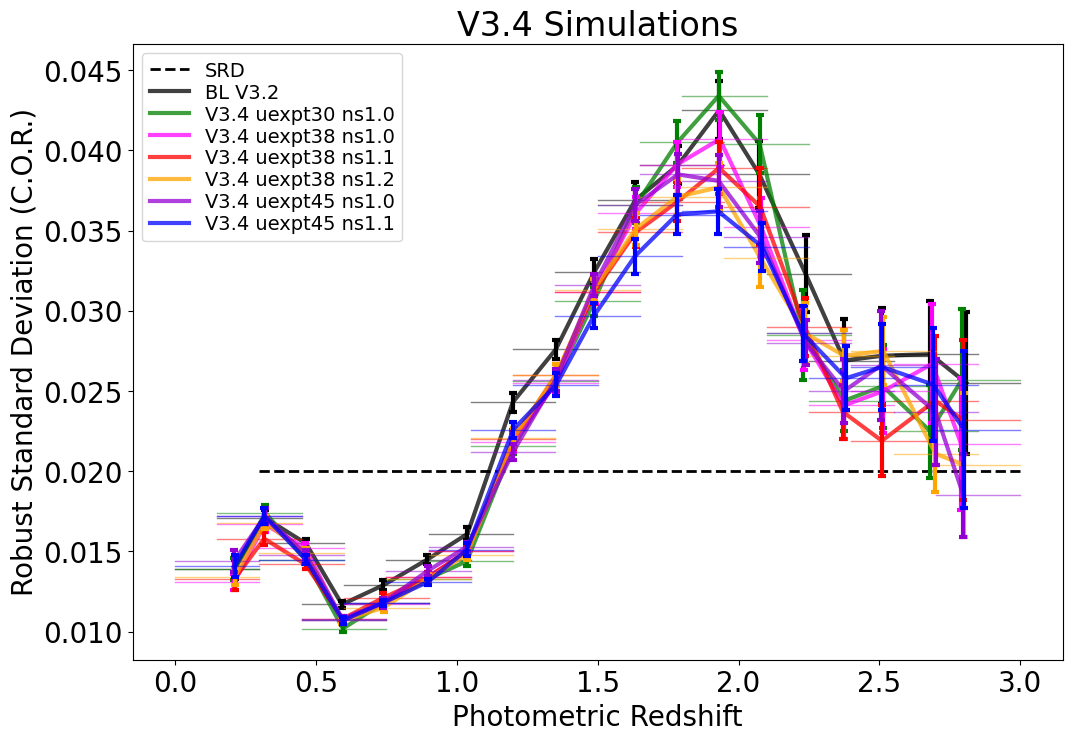
\includegraphics[width=0.42\textwidth]{figures/photo-z.png}
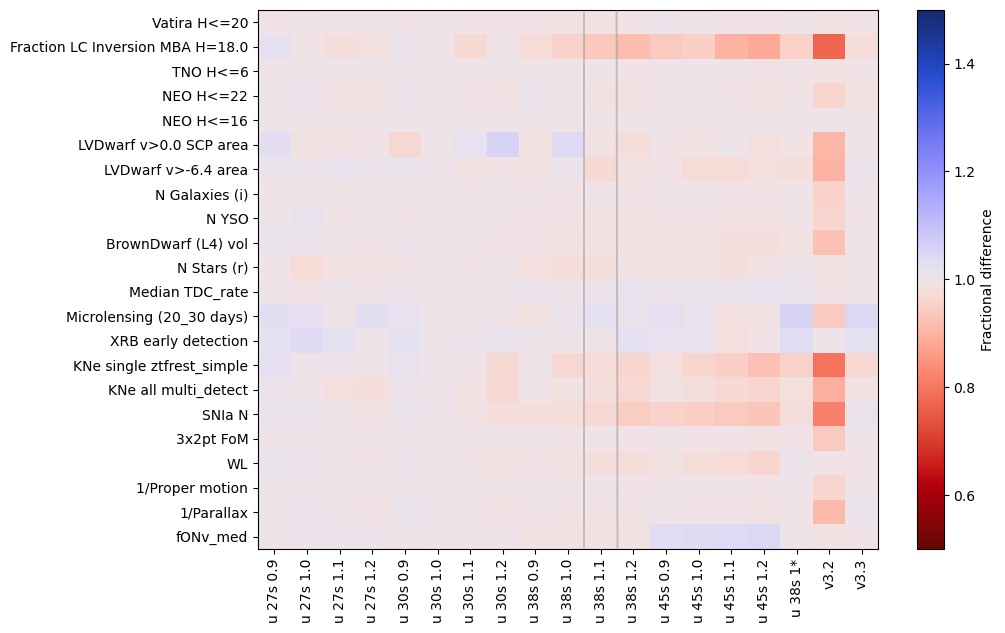
\includegraphics[width=0.47\textwidth]{figures/u_band_scoc_heatmap.png}
\caption{\emph{Left}: Effect of changes of $u$-band 10-year depth on \pz\ Roubst Standard deviation as a function of redshift $z$ as measured in \cite{Graham_2017}. The dashed line represents the \citetalias{LPM-17} requirements on \pz. The black solid curve is the \baseline{3.2}, the latest baseline before the filter transmission curves were updated in the Rubin simulation system, the colored curves represent the \pz\ Robust Standard Deviation varying $u$-band exposure time between $30\leq u_{expt} \leq45$~seconds and number of exposures in $u$ band between $1.0\times ns \leq N_u \leq 1.1\times ns$ where $ns$ is the number of $u$-band exposures in \baseline{3.2}. A similar impact is seen in \pz\ bias. \emph{Right}: a standard set of science and system MAFs metrics as a function of changing exposure time ($27\leq u_{expt}\leq 60$ seconds) and fraction of exposures in $u$ band ($0.9\times ns\leq N_u \leq1.5\times ns$). The metrics are normalized with respect to a simulation with $u_{expt}$= 30 seconds and $N_u = 1.0\times ns$. Three additional columns in the end show the $v_3.2$ (\baseline{3.2}, pre-filter-throughput update) and $v3.3$ (\baseline{3.2}, similar simulation to \baseline{3.2} but baseline after throughput updates) and $u~38s~1*$. In all other simulations shown in this plot the exposure time in all bands by $u$ is kept at 30 seconds, whereas in this simulation to compensate for the added time in $u$ band ($u_{expt}=38$~seconds) the other bands have decreased exposure time of 29~seconds (which is the current implementation the SCOC recommends for \baseline{4.0} and the standard implementation in simulations $v3.5$ and later).}

\end{figure}
\FloatBarrier

\subsection{Rolling}\label{sec:rolling}
In a rolling strategy, instead of distributing visits uniformly on the WFD footprint, the sky is split into regions that alternate high- and low-intensity monitoring. In \citetalias{PSTN-055}, the SCOC recommended the implementation of a rolling strategy for the LSST WFD at a strength of 0.9\footnote{This number represents the fraction of the visits that the scheduler attempts to place in the high-activity rolling region. However, the resulting visit distribution is more uniform (75-80\% in high-activity regions, 25-20\% in low ones) due to competing requirements (\eg , filter balance, minimum number of observations per pointing per year in each filter to produce templates, weather, etc...)} 
with the sky split into two rolling regions constituted by four longitudinal stripes. The primary drivers for this recommendation are time-domain science including the exploration of the transient and variable sky and SN cosmology. Rolling as described decreases the median time-gaps compared to a no-rolling implementation of LSST:
distributing the $\sim$800 visits per pointing evenly into 10 seasons results in an median revisit time per pointing of about 4.5 nights, while rolling can increase the cadence on the areas of sky closer to 2.5 nights.\footnote{The reader is reminded that each pointing receives two or three visits per night. The time gaps reported here are for inter-night observations.}

 However, concerns were raised by the DESC, and seconded by other groups such as the Galaxies SC, regarding the lack of uniformity in the distribution of depths across the survey at intermediate years between 1 and 10 compared to a no-rolling strategy \citep[see discussion in][which noted this as a potential future concern before the adoption of a rolling cadence as the baseline]{2022ApJS..259...58L}.  These concerns highlighted the negative impact that rolling induces on the cosmological analysis conducted with static-sky probes due to a decreased uniformity of the data releases, which has been shown to cause several significant issues for cosmological large-scale structure analyses \citep[\eg ,][]{2022PhRvD.105b3520A,2023JCAP...07..044B}.  
 This uniformity challenge could be addressed after data collection by selecting and limiting the number of images going into a data release per field (including these data in future data releases) to achieve higher uniformity or by a ``renoising'' step. These data management solutions are at the moment unscoped and do not fall under the current requirements of the Rubin DM deliverables.

 \begin{quote}
     [\citetalias{PSTN-055}] ``The current SCOC recommendation is to implement a rolling cadence with a half-sky rolling scheme and a 0.9 rolling weight. However, rolling impacts the uniformity of static data releases which, as experts in the community have highlighted, is necessary for static sky science in general and cosmology in particular. This issue may be resolved or mitigated at the software level in the creation of coadds and catalogs, rather than at the scheduler level. The community should specify the desired and necessary requirements for uniformity to enable the exploration of data processing solutions to this problem. Depending on the feasibility of a solution to ensure sufficient uniformity, the SCOC recommendation on rolling may be re-evaluated.'' 

 \end{quote}

 With the goal of quantifying the necessary uniformity to enable cosmological results at certain key data releases\footnote{These intermediate releases were selected because they enable equally-spaced time intervals between new datasets for comprehensive static science analysis: years 1, 4, 7, and 10 corresponding to DR2, DR5, DR8, DR11.}, DR5 and DR8, as well as identifying solutions that enable rolling (at the strength recommended in \citetalias{PSTN-055}) while increasing the uniformity of key data releases, a Uniformity Task Force developed alternative rolling implementations. {\it Uniform rolling}, implements interruptions of rolling before specific data releases to increase the uniformity of those releases and recover an acceptable level of uniformity at key years -- see Figs.~\ref{fig:stripiness} and~\ref{fig:uniform-rolling}.  It was found that uniform rolling permits the full survey area to be used for cosmological analysis at years 4 and 7, whereas in previous rolling versions, approximately 35\% of the cosmological constraining power\footnote{Here we quantify cosmological constraining power through emulated forecasts of combined constraints from cosmological weak lensing and large-scale structure measurements \citep{2022ApJS..259...58L}.  The constraints assume a $w_0 w_a$CDM cosmological model, with $w_0$ and $w_a$ entering as two parameters in the dark energy equation of state.  The constraining power is quantified through the area of the uncertainty contours in the $(w_0, w_a)$ part of parameter space, marginalizing over other cosmological parameters and systematic uncertainties -- then taking the inverse of that area (so that higher values mean lower uncertainty, i.e., tighter cosmological constraints).  However, this can be considered more generally as a proxy for how well we are measuring cosmological structure growth, translating into tighter constraints on the amplitude of matter fluctuations if a $\Lambda$CDM cosmological model is assumed.} was lost at those years due to the need for area cuts. 

We note that rolling can be implemented with at most four rolling cycles (that is, starting rolling in Y2 and ending rolling in Y10) where a cycle is defined as a pair of two years where the high- and low-intensity regions are swapped. Uniform rolling requires limiting rolling to three cycles. Primarily this affects science sensitive to timescales of $\sim24-48$ hours \footnote{Shorter time scales are primarily covered by observations in triplets as discussed in \citetalias{PSTN-055}.}. 
We note that these time scales had been identified as sensitive and requiring additional improvements in \citetalias{PSTN-055} within the recommendation on rolling (PSTN-055 Section 2.4.1): 

\begin{quote}
``[\citetalias{PSTN-055}] the SCOC recommends the LSST cadence
be designed to ensure coverage of time scales in the hours-to-one-day range by carefully tuning survey parameters in combination. Performing three visits per night by default is not recommended, but a combination of preferentially pushing a third visit to the following night [...] and requesting a third visit within a night once every several nights ($\sim 1$ week) would achieve this goal.'' 
\end{quote}

While not designed for this purpose, the implementation of the 0.9 strength, two-sky-areas rolling with four cycles (\baseline{3.2} and later) improved coverage at 24-48 hours (see figure \autoref{fig:rolling_sampling}).


\begin{figure}
    \centering
    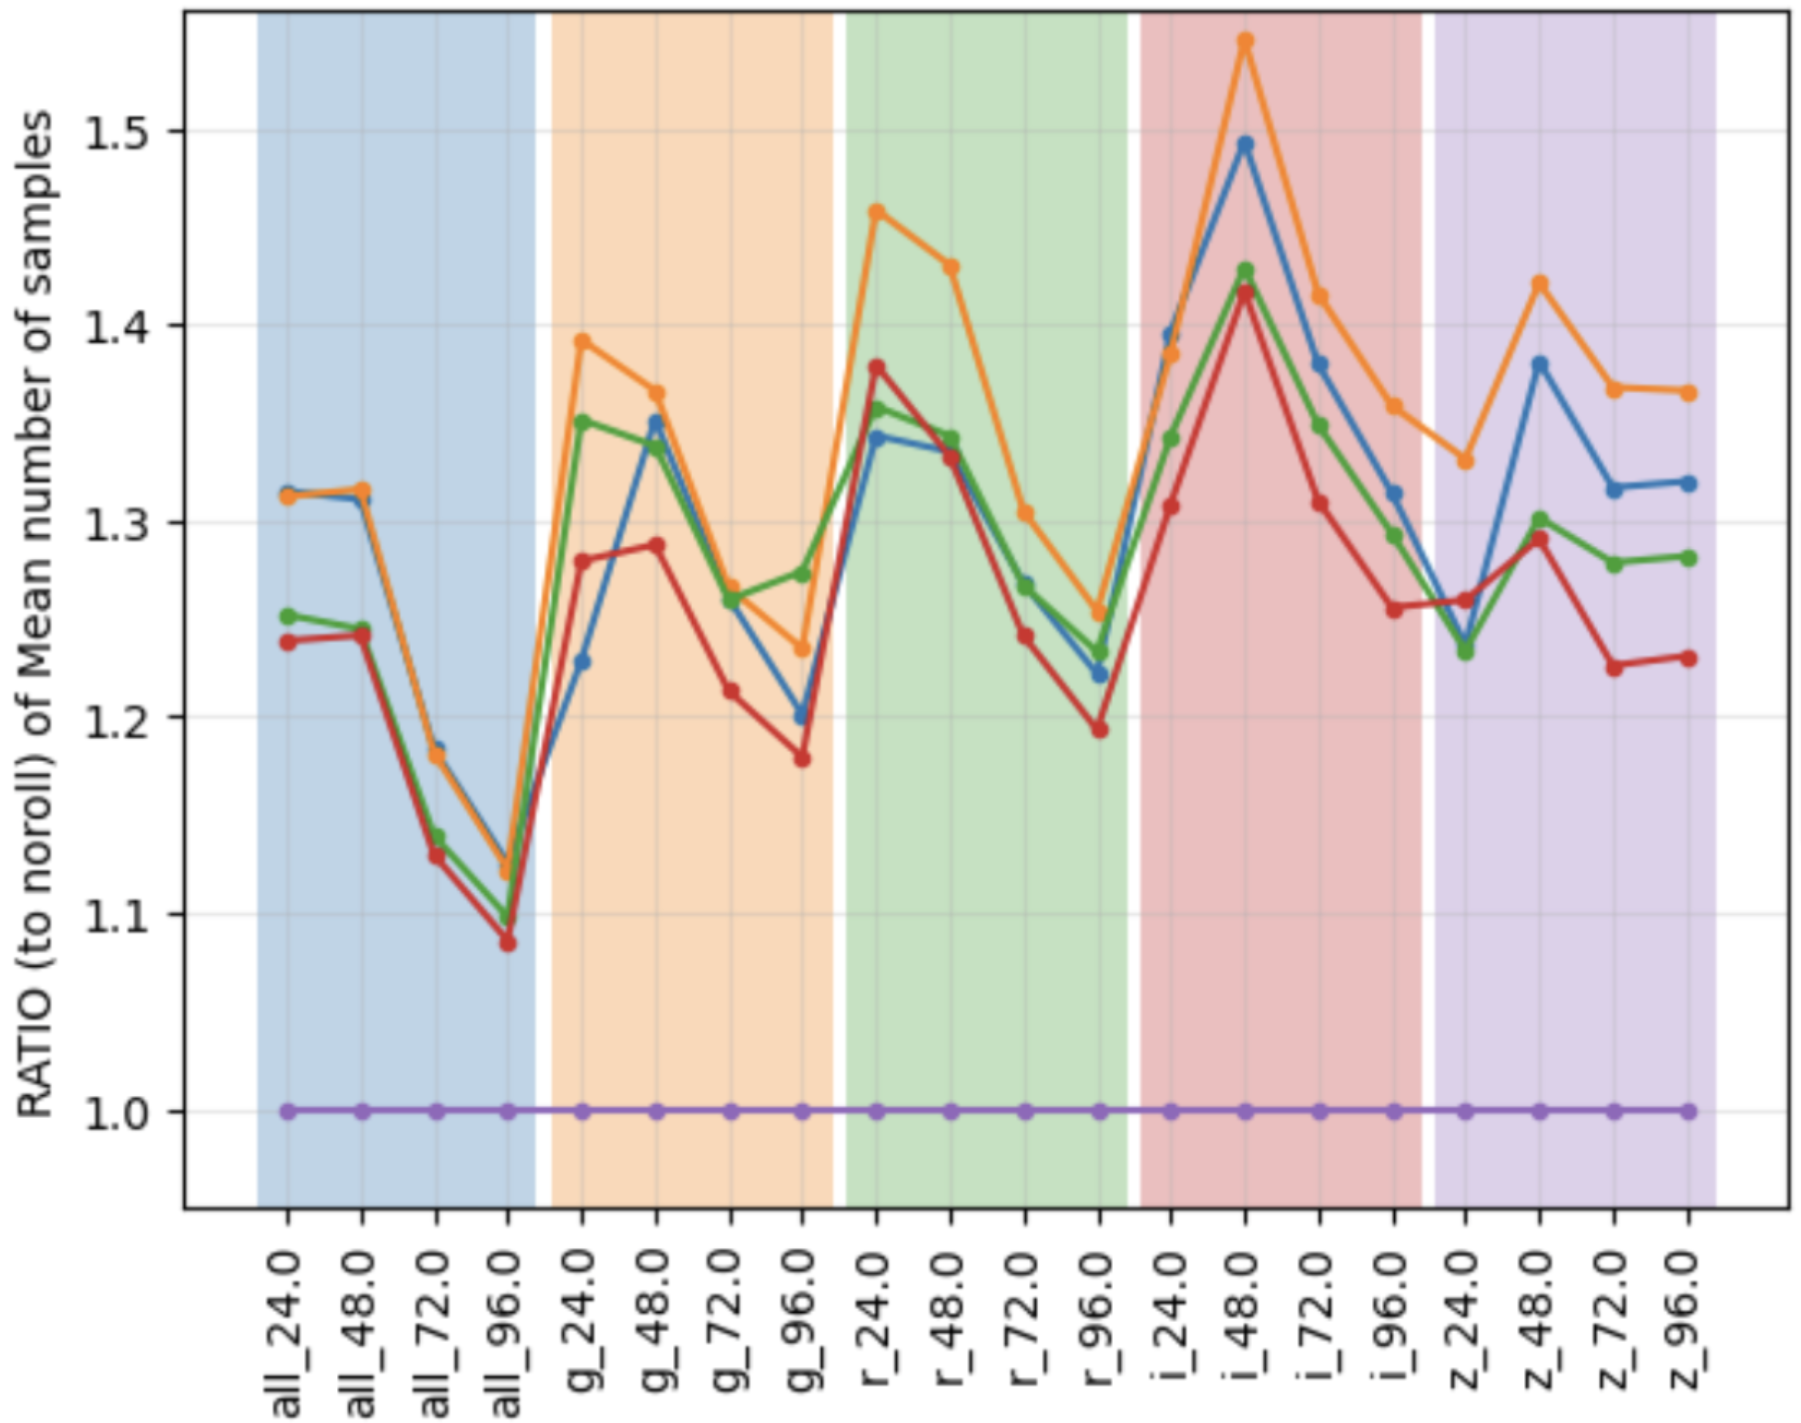
\includegraphics[width=0.4\linewidth]{figures/rolling_sampling.png}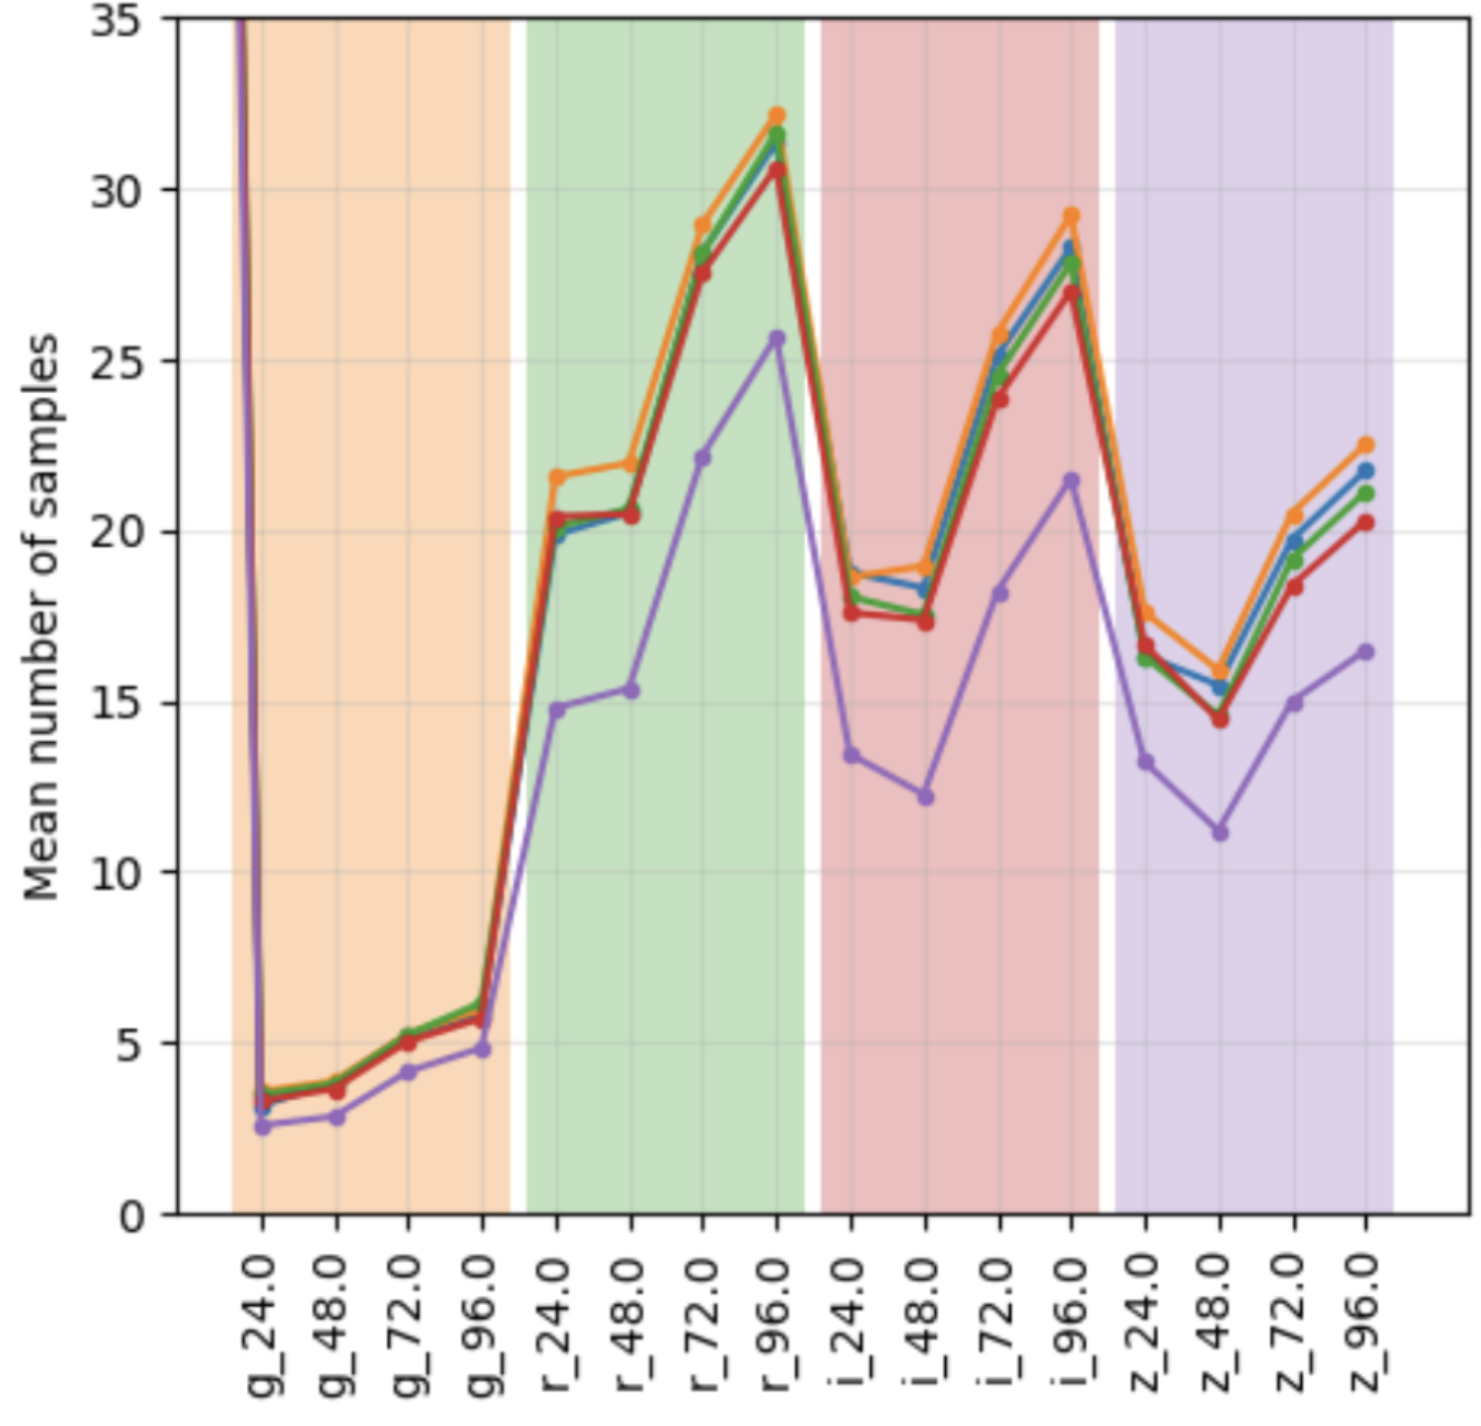
\includegraphics[width=0.58\linewidth]{figures/rolling_nsamples.png}
    \caption{The mean number of observations at 24, 48, 72, and 96 hours in all bands, $g$ band only, $r$ band only, and $z$ band only as a function of the number of rolling cycles: each cycle of rolling cadence improves the number of samples by about 7\%. On the left, the ratio of samples normalized to the number of samples when not rolling is shown for two \opsim s with 3 rolling cycles (\texttt{roll\_3\_v3.4\_10yrs} and \texttt{roll\_uniform\_early\_half\_mjdp0\_v3.4\_10yrs}) and two \opsim s with 4 rolling cycles (\baseline{3.3} and \baseline{3.4}). On the right, the absolute number of samples is shown in $g$, $r$, and $i$. Note the overall small numbers of samples in these time scales when not rolling: $<5$ in $g$ and  $10<ns< 15$ in $r$, $i$, $z$ at 24 hours. The rolling strategy improves sampling between 24 and 96 hours, but recall that \citetalias{PSTN-055} concluded that the sampling enabled by the rolling as implemented in \baseline{3.0} (in three cycles) was still insufficient. A fourth cycle of rolling improves this sampling by $\sim7\%$.}
    \label{fig:rolling_sampling}
\end{figure}

The SCOC recognizes the positive impact this rolling implementation has on static cosmological and extragalactic probes and considers this a promising solution for the uniformity concerns raised in \citetalias{PSTN-055}, with limited impact on time-domain probes. However, this implementation of rolling is a significant and new departure from earlier implementations, and the number of cycles of rolling had not been previously explicitly discussed as a parameter in the survey strategy. Furthermore, the current Uniform Rolling implementation requires rolling to start early in Y2 (in the current implementations rolling starts on survey day $\leq 400$) but, as discussed in \citetalias{PSTN-055}, rolling shall not start until sufficient sky coverage has been achieved to enable proper photometric calibration\footnote{\tbd{A discussion and references for "good enough" calibration should be added, see Eli 2023 PCW - @fed}}. 

For these reasons, the SCOC is not committing at this time to recommend any specific implementation of rolling, beyond confirming the strength 0.9 and two-region strategy. Since in all current implementations
rolling does not begin until Y2, the SCOC intends to continue investigating rolling implementations and their impact throughout Y1, with the support of the community, and release a recommendation of how to implement rolling in its first annual recommendation ahead of Y2 of Operations. In particular, we intend to (1) investigate sensitivity to the outcomes of Y1, (2) ensure the community has time to evaluate the potential impacts of these changes that are not currently highlighted by our metrics, and (3) refine the uniform rolling implementation details.

{\it The SCOC recommends that the time domain community, particularly those interested in phenomena that have evolutionary time scales of hours-to-days, urgently quantifies the impact of the proposed uniform rolling compared to rolling in four cycles. For this purpose, while the baseline is implemented with 3-cycles uniform rolling, the Survey Strategy team has prepared v3.5 \opsim s  with different rolling implementations.}

{\it Further, the SCOC iterates the recommendation that Data Management scopes a plan for producing uniform data releases in DR5 and DR8 in addition to the standard data releases and that the cost of the development and storage of these additional data releases is scoped and shared with the scientific community.} Even if produced by the Rubin DM, uniform data releases will require the input (of the DESC and extragalactic science community at large) to develop the algorithm that will achieve sufficient uniformity. Understanding the cost of producing two additional {\it uniform} data releases is necessary to compare this cost to the scientific cost of three vs four cycles of rolling, to be measured by the community (see previous paragraph). In addition, if rolling cannot start early enough to interrupt rolling ahead of DR5 and DR8, this remains the only alternative solution currently identified to achieve sufficient uniformity. Sharing information on the cost of additional data releases will place the community in a position, if needed, to advocate and secure funding for this purpose.

The SCOC is thankful to the Uniformity Task Force, chaired by Rachel Mandelbaum, which provided invaluable contributions and analysis that led us to this recommendation.

%\tbd{ NOTE: we should add direct answers to these questions: Rachel? The community should specify the desired and necessary requirements for uniformity to enable the exploration of data processing solutions to this problem. Depending on the feasibility of a solution to ensure sufficient uniformity, the SCOC recommendation on rolling may be re-evaluated.}  \tbd{From Rachel: There isn't a single number we can give regarding requirements.  Would it be sufficient to say that the uniformity task force has provided quantitative metrics (some heuristics, some truly science-driven) that address this recommendation?}

\begin{figure}
    \centering
    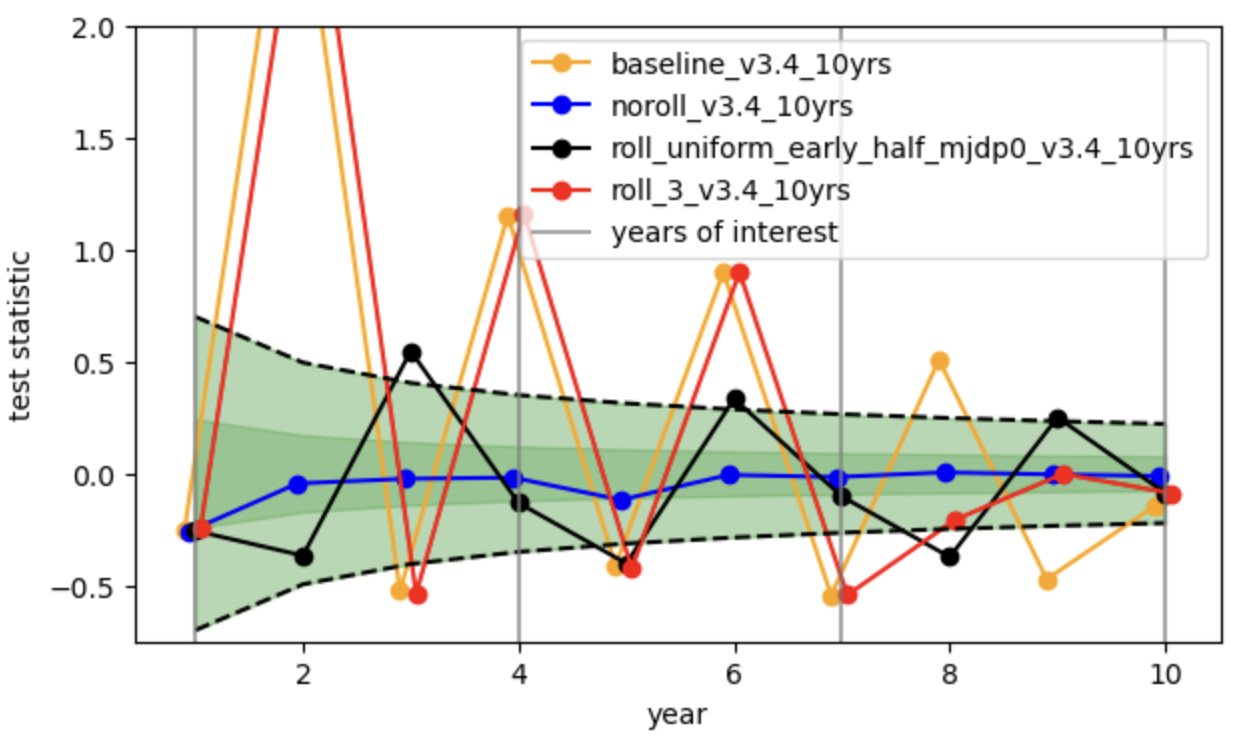
\includegraphics[width=0.7\linewidth]{figures/stripiness_metric.png}
    \caption{
    Quantitative assessment of the non-uniform exposure time variation vs.\ year under different observing strategies.  The test statistic plotted on the vertical axis effectively measures the fractional difference between the variations in depth between the northern and southern Galactic regions, with a value of 0 indicating that the two are the same, as expected for a perfectly uniform survey.  The light green shaded envelope between the dashed black lines indicates the region for which we consider the stripe features to be negligible (meaning manageable within the limits of existing analysis algorithms).   The narrower dark green shaded envelope shows the expected statistical fluctuations for a survey without rolling, as estimated using the \texttt{noroll\_v3.4} strategy simulation.  As shown, at the highlighted years (1, 4, 7, 10) the uniform rolling strategy (\texttt{roll\_uniform\_early\_half\_mjdp0\_v3.4\_10yrs}) is very close to uniform within the level of statistical fluctuations at Y4 and Y7 (DR5 and DR8), while the \baseline{v3.4} strategy is highly non-uniform, especially in those years.
}
    \label{fig:stripiness}
\end{figure}

\begin{figure}
    \centering
    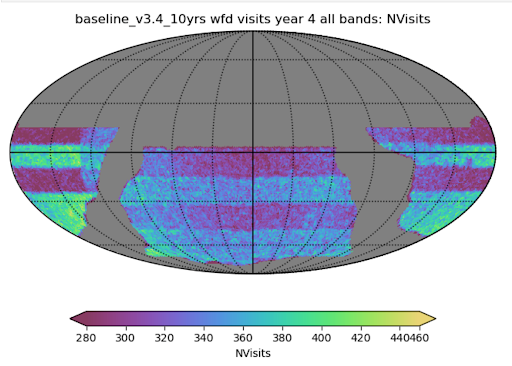
\includegraphics[width=0.3\linewidth]{figures/Rolling.png}
    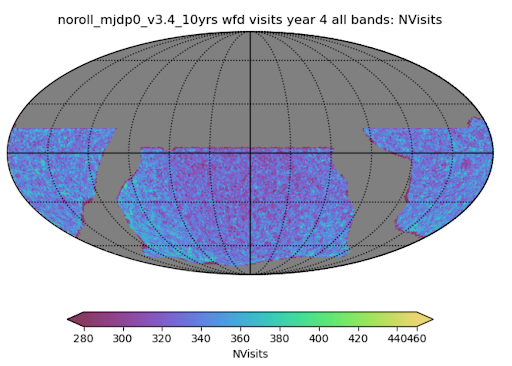
\includegraphics[width=0.3\linewidth]{figures/RollingCompare.png}
    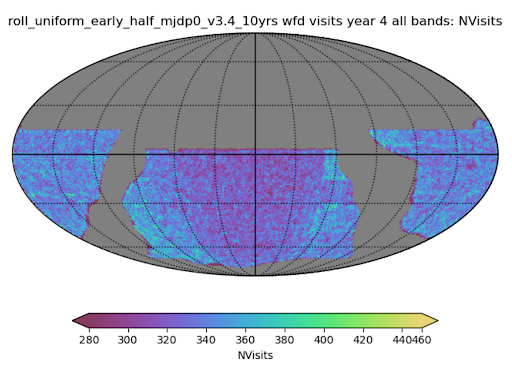
\includegraphics[width=0.3\linewidth]{figures/RollingUniform.png}
    \caption{
Comparison of the depth of LSST at the end of Y4 (DR5) under different rolling strategies. The left plot shows the LSST number of visits map for a standard implementation of rolling at strength 0.9 in two sky regions designed as four longitudinal stripes. The center plot represents an implementation of LSST without rolling, for comparison and provides an upper limit to expected uniformity. The right plot shows the implementation of Uniform Rolling described in this section and implemented in \baseline{4.0}.}
    \label{fig:uniform-rolling}
\end{figure}

\FloatBarrier


\subsection{Galaxy}\label{sec:galaxy}
In \citetalias{PSTN-055} the SCOC identified areas of work needed to finalize the WFD survey strategy on the Galactic sky and special regions of interest to Galaxy science, including the Clouds and South Celestial Pole, which can be observed within the WFD but with different observing choices than the low-dust footprint, of primary interest for extragalactic science. This section includes updated recommendations on the Galactic footprint and its observing cadence, including whether rolling should be implemented (\autoref{sec:subG:footprint}), filter balance (\autoref{sec:subG:filterbalance}):
\begin{quote}
    [\citetalias{PSTN-055}] The SCOC is not ready to finalize a recommendation for the
filter balance in the Galactic Plane, or for a final Galactic Plane/Bulge footprint, or the rolling scheme to be implemented on the Galactic Plane. The SCOC will work with the SMWLV and TVS SCs to ascertain the best solutions for Galactic science on filter balance and footprint. These decisions should, however, not impact decisions relating to the WFD and the time spent collectively on Galactic regions should not change.
Galactic Plane pencil-beam surveys need to be defined more clearly to assess if they would ultimately result in ``nano-surveys'', which will require a fraction of time too small to be optimized at this stage, or to evaluate the possibility of incorporating them in a final Galactic Footprint recommendation.



\end{quote}and special regions (\autoref{sec:subG:specialregions}).

\subsubsection{Footprint and Time Distribution of Visits}\label{sec:subG:footprint}

Extensive work has already led to the present division of the dense regions of the Galaxy into a high-visit region that encompasses both a large area around the Bulge and a long, thick strip of the Plane, surrounded by a larger area in the Plane with fewer visits. %This division was needed because the overall survey constraints prevent covering this entire area at WFD depth. 
The subsequent efforts of the SCOC and scientific community have been focused on refining these choices.

One feature of the \baseline{3.0} (\citetalias{PSTN-055}) survey in the Plane is that it left a high-visit ``blob'' centered around a Galactic longitude of $l=+45$ surrounded by a lower visit area. This resulted from a previous candidate survey design that included high-visit pencil beams\footnote{In a subset of previous candidate survey designs, ``pencil beams" were a series of 20 high-visit single pointings distributed in galactic longitude with the goal of ensuring the survey sampled a range of stellar environments.} at varying Galactic longitudes along the Plane and considered stellar density, but was not due to any other specific science goal in this region. Visits centered around this high-declination blob would necessarily have to occur at high airmass, and would additionally be separated from other high-visit areas, reducing survey efficiency.

{\it The SCOC recommends redistributing the excess visits in the ``blob'' centered around a Galactic longitude of $l=+45$ to cover a low-visit ``barrier'' at $l=+335$ in the Plane and at the border of the Plane and Bulge. This change would give continuous longitude coverage along the Plane from a longitude of $l=+30$ down through $l=+280$ and boost metrics for time-domain science in the Bulge/Plane.}


\begin{figure}
\centering
    %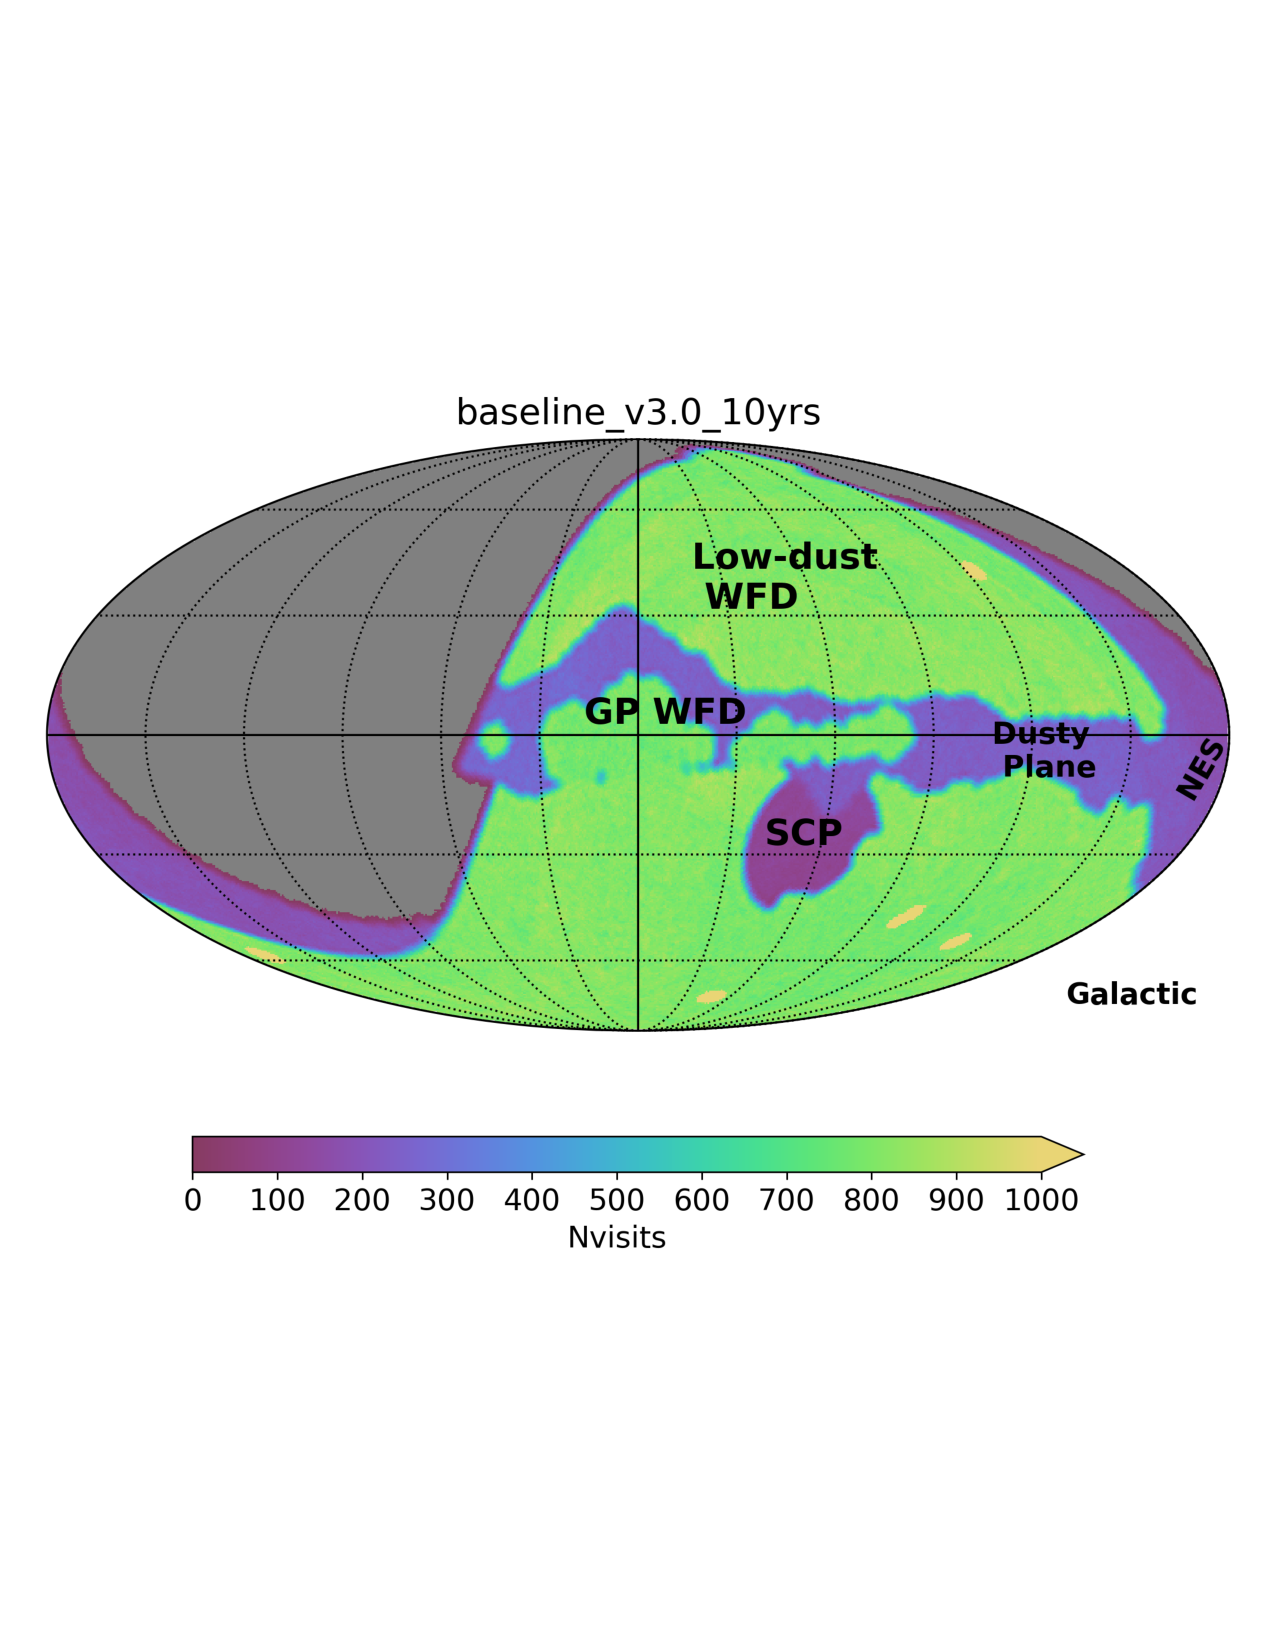
\includegraphics[width=0.75\textwidth]{figures/baseline_v3.0_10yrs_nvisits_galactic.pdf}
    %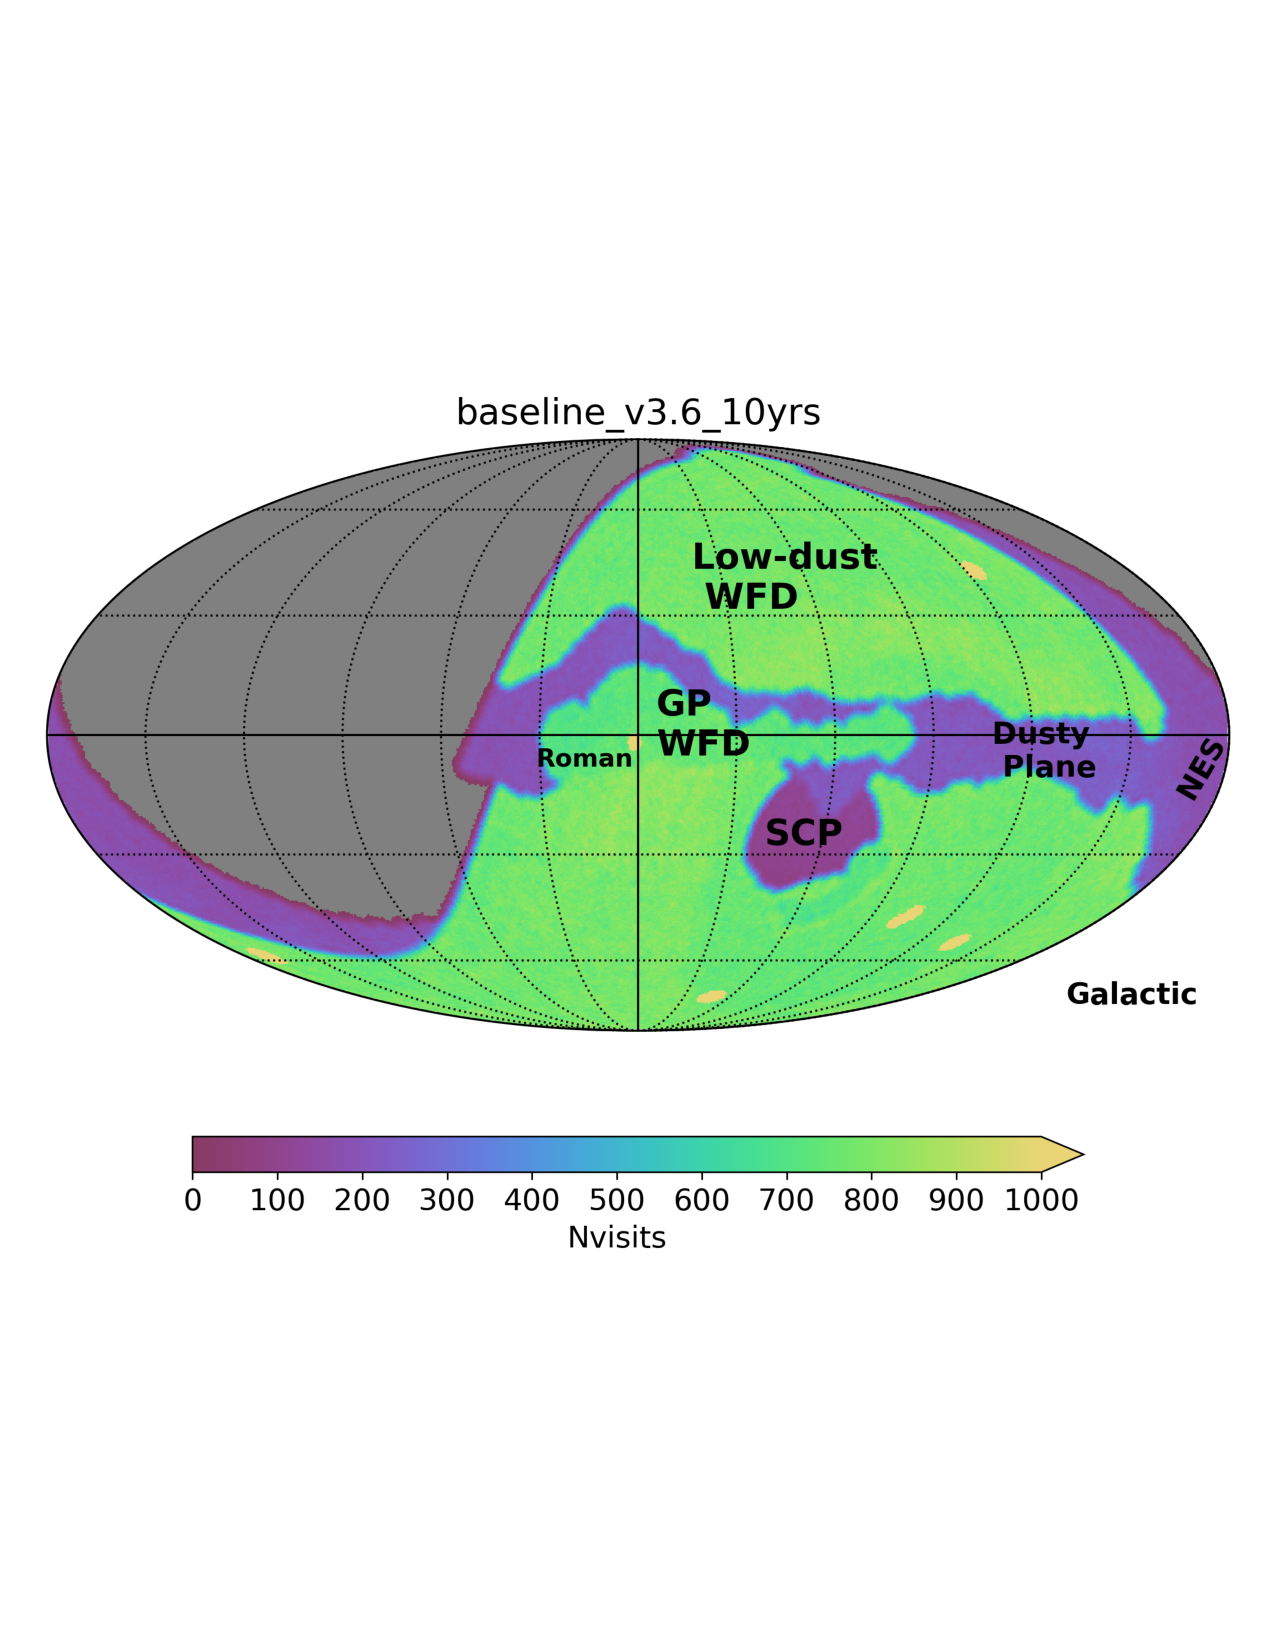
\includegraphics[width=0.75\textwidth]{figures/baseline_v3.6_10yrs_nvisits_galactic.pdf}
    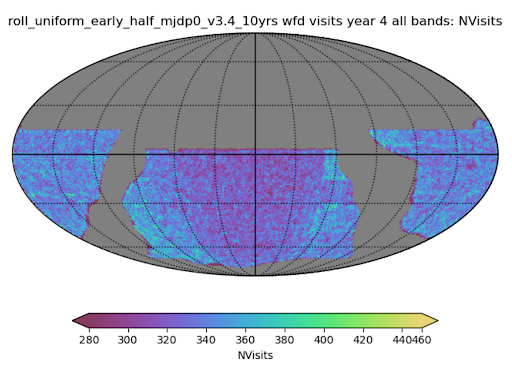
\includegraphics[width=0.3\linewidth]{figures/RollingUniform.png}
    \caption{Comparison of the MW footprint (Galactic coordinates) as recommended in \citetalias{PSTN-055} and implemented in \baseline{3.0} and through v3.5 simulations and the refined footprint recommended in this document and implemented in \baseline{3.6} and later.}
\end{figure}

The SCOC recommends rolling on the low-dust WFD (see \autoref{sec:rolling}), where strips in declination alternate high- and low-intensity monitoring. %Rolling trades detection of transients for improved temporal coverage; for some classes of extragalactic transients, such as SN Ia to be used for cosmology, this tradeoff is strongly positive on net.
However, this rolling implementation need not extend to the dense regions of the Galaxy, if it does not provide overall scientific benefits to Galactic science.

In \baseline{3.0}, no rolling is implemented in the Bulge and Plane footprint. The SCOC explored simulations that implemented rolling in both regions or in only the Bulge.
Rolling in both the Bulge and Plane is extremely unfavorable for many Galactic transient metrics, such as microlensing discovery and characterization for a broad range of event timescales, as well as early detection of X-ray binary outbursts.\footnote{The X-ray binary outburst metric is representative of Galactic transients with a typical duration longer than a few days that follow the stellar distribution in the Galaxy, so has much broader relevance than solely for X-ray binaries.} The outcomes are more complex for rolling in the Bulge alone; while still negative for Galactic transient discovery, rolling in the Bulge has a mixed effect on microlensing metrics. These Bulge simulations particularly aimed to explore whether rolling cadence implementations could boost the early detection and characterization of shorter ($\sim$ few days) timescale microlensing events and anomalies, even if only for a limited survey region. In practice, the improvement was found to be comparatively small, and came at the detriment of the regular, long-baseline monitoring necessary to characterize long-timescale events such as those caused by compact object lenses.   


{\it The SCOC concluded that rolling on the Galactic footprint would have a net negative effect on the survey as a whole, and recommends no rolling in the Plane or Bulge.}

Finally, the SCOC recommends redistribution of a small number of Bulge visits to 
a central Bulge field overlapping the planned Roman Bulge survey area, with a goal of more continual monitoring to improve microlensing detection and characterization in this region that will be intensively surveyed by Roman during predetermined seasons.
This recommendation was first implemented in \opsim\ \texttt{roman\_v3.3} and resulted in large improvements for some microlensing metrics, improvements for all microlensing metrics, and no significant negative impact on any other metrics. 

{\it The SCOC recommends that a visit plan consistent with this \texttt{roman\_v3.3} with the number of redistributed visits to be capped at that used in this simulation: in the current Roman field \opsim s the number of visit reallocated to the Roman field is $\sim1600$. However, the timing of the implementation of this augmented observing campaign needs to remain flexible at this time to respond to the as-of-yet to be finalized launch date of Roman and the scheduling of its surveys.}


\subsubsection{Galactic Filter Balance}\label{sec:subG:filterbalance}

The filter balance in the Bulge in the current \baseline{3.4} already differs from that used for WFD: the primary difference is fewer visits in $y$, which are redistributed to bluer filters to better optimize Galactic science since $u$ and $g$ are vital for stellar characterization even in the presence of foreground dust. In WFD $y$ receives a large number of visits, comparable to $z$ and only slightly less than $r$ or $i$, while $g$ and especially $u$ receive fewer visits. Hence $y$, with its relatively low sensitivity, is the optimal choice for redistribution to bluer bands.

Noting the relatively low sensitivity of the $y$ band, and its resulting negligible reddening advantage over $z$ even in dusty regions, the SCOC considered several simulations that redistributed additional visits in the dense regions of the Galaxy from $y$ to a combination of $z$, $g$, and $u$, while still recognizing the fundamental discovery potential of a multi-filter survey over a broad contiguous area. The main finding from these new simulations was that most existing metrics showed mixed or marginal changes, even where the relative number of visits in $u$ and $g$ substantially increased. The metrics considered included Galactic transients, young stars, detection of several classes of periodic variables, light curve gaps, as well as solar system metrics (since the ecliptic passes through this region).

{\it The SCOC finds that the adoption of a revised filter balance in the Bulge and Plane with less $y$ and more $z$, $g$, and $u$ compared to the present baseline is potentially beneficial on the net, but that existing metrics are not adequately sensitive to the explored filter balance changes for some expected science cases. The SCOC concludes that a survey using the currently implemented filter balance in the Bulge and Plane in \baseline{3.4} will produce excellent science and the LSST can start with this implementation.} 
However, the SCOC also welcomes input from the community whose science is affected by the details of filter balance in the dense regions of the Galaxy to help define improved metrics that could lead to further optimization in future years.


\subsubsection{The Milky Clouds and South Celestial Pole}\label{sec:subG:specialregions}

The scientific goals of the survey in the region of the Large and Small Milky Clouds (LMC and SMC, together MCs)\footnote{There is an effort underway to have the community avoid using the name Magellanic Clouds, as reasoned in \url{https://physics.aps.org/articles/v16/152}. Milky Clouds has been proposed as an alternative and has indeed been used in a number of settings. We adopt this name here to reflect the broad and inclusive reach of Rubin LSST.} and South Celestial Pole (SCP) differ somewhat from WFD. In particular, the major areas of focus of the survey of the main bodies of the LMC and SMC are microlensing and other variable/transient science. In the peripheries of the MCs, including the South Celestial Pole region, the central goal is to detect dwarf satellites and other low surface brightness stellar substructures.
These goals are supported in the current baseline, as the MCs are covered with visit numbers like that in WFD, while the SCP region, only observable at relatively high airmass, has a low number of total visits, but sufficient to detect many potential dwarf satellites and substructures. However, the current baseline also adopts the WFD filter baseline in the MC and SCP regions, which may not be ideal for the stated goals.


A number of simulations were considered that used an alternate filter balance for both the Clouds and the South Celestial Pole, moving visits out of $z$/$y$ and toward $u$/$g$ in both regions. These simulations show large improvements in metrics relevant to the detection of low surface-brightness dwarfs as well as some improvements in microlensing and variable star/transient metrics. 

{\it The SCOC recommends a bluer filter mix in these regions, bounded by the requirement that the increased number of dark-time visits in a relatively narrow range of right ascension does not affect other parts of the survey.} 

\begin{figure}
    \centering
    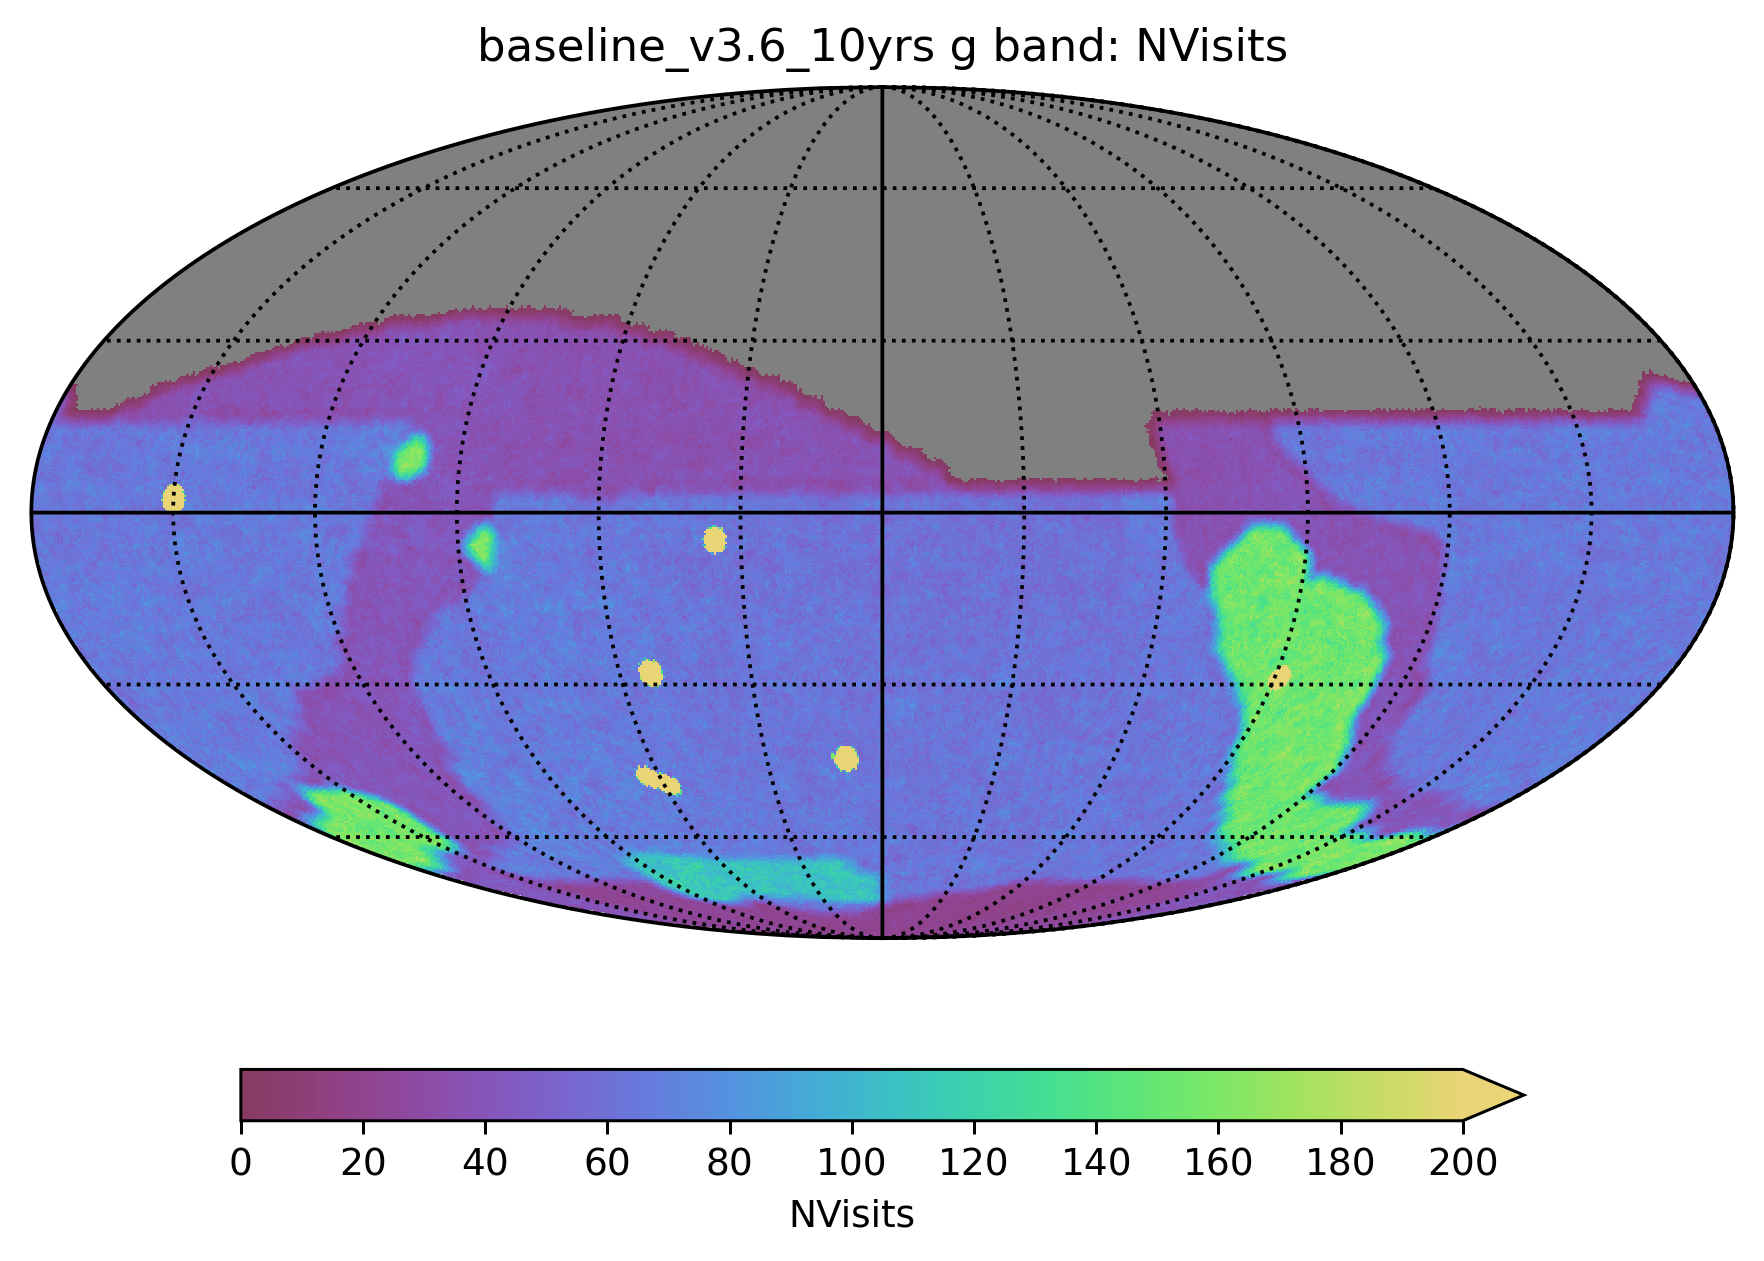
\includegraphics[width=0.32\linewidth]{figures/baseline_v3_6_10yrs_NVisits_g_band_HEAL_SkyMap.png}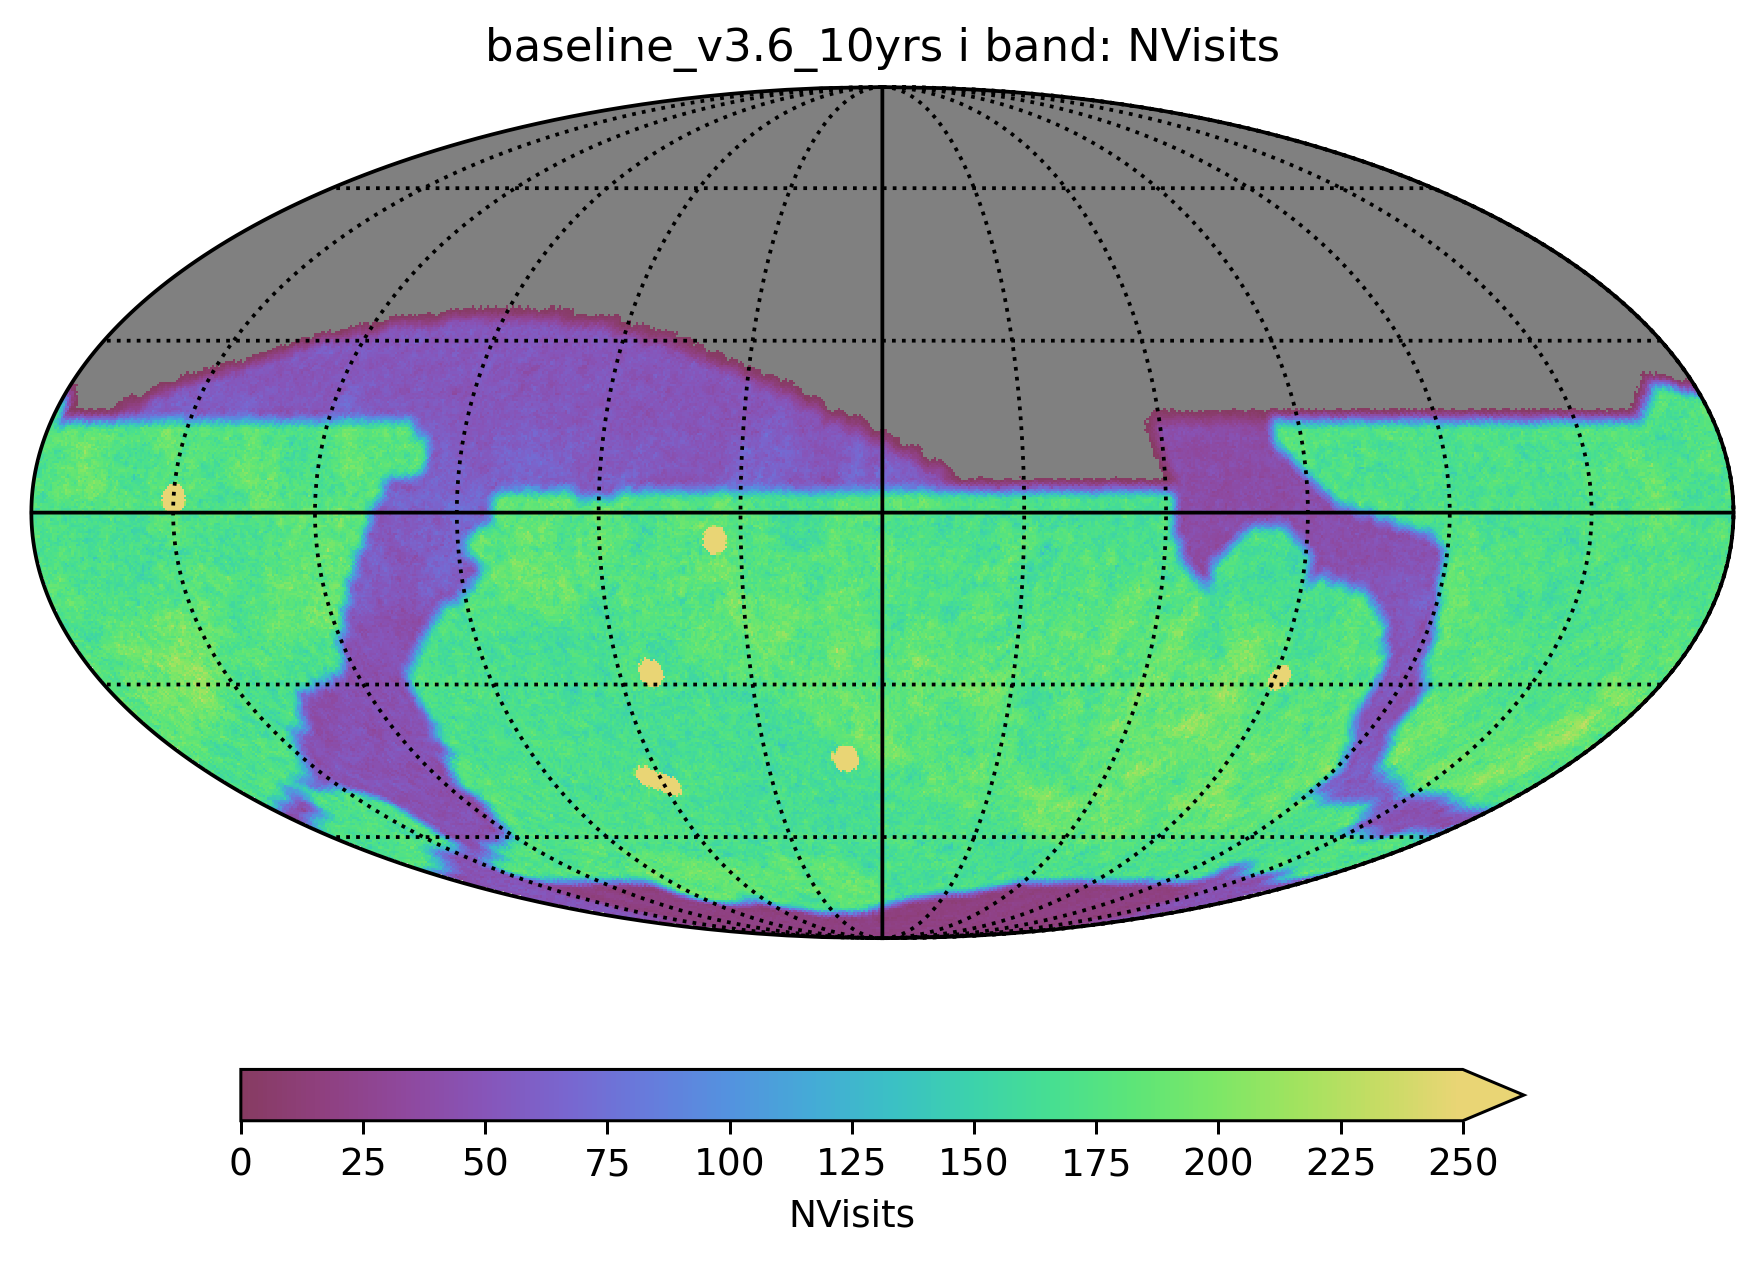
\includegraphics[width=0.32\linewidth]{figures/baseline_v3_6_10yrs_NVisits_i_band_HEAL_SkyMap.png}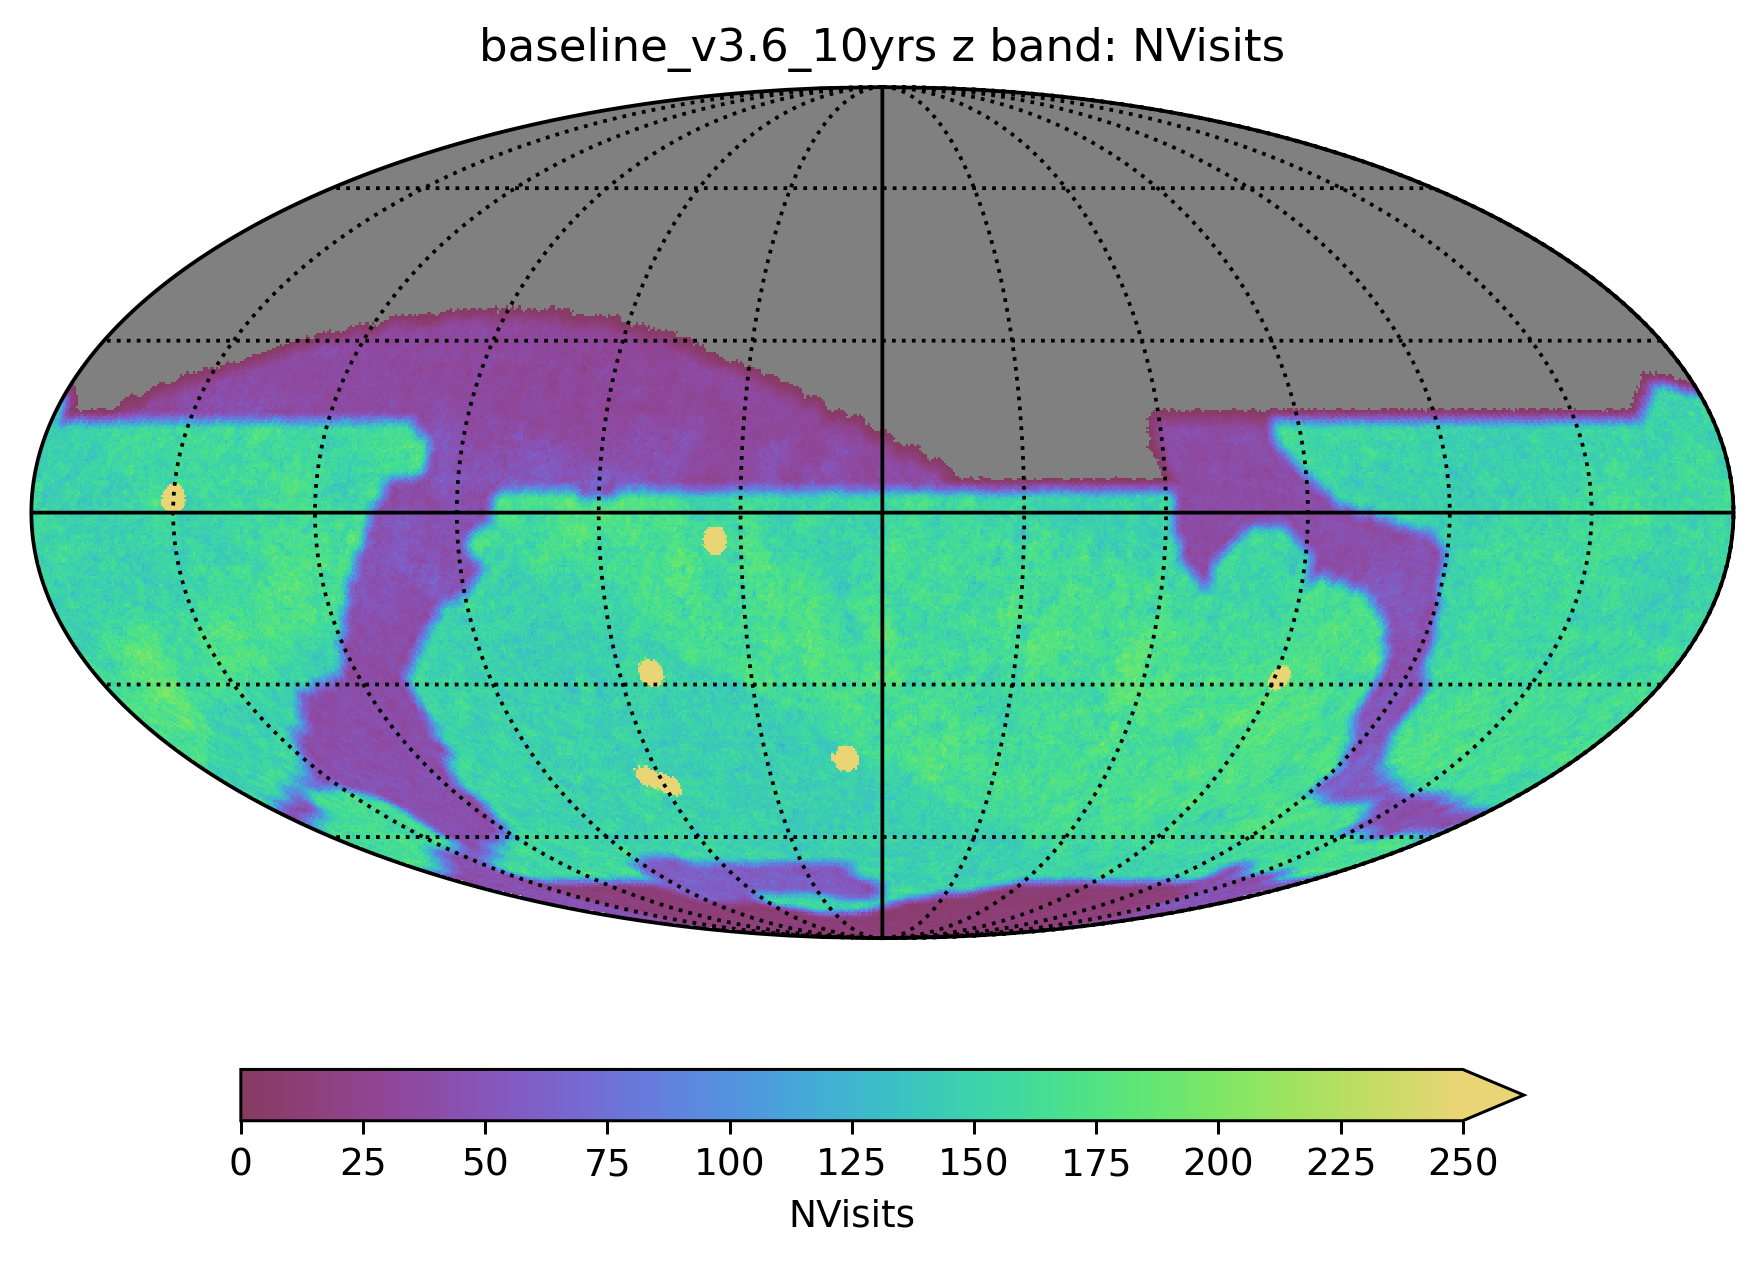
\includegraphics[width=0.32\linewidth]{figures/baseline_v3_6_10yrs_NVisits_z_band_HEAL_SkyMap.png}
    \caption{The different filter balance in the LMC and SMC region compared to the rest of the WFD can be seen when comparing the number of exposures in $g$, and $i$, and $z$ at the end of the 10 year survey (the rectangular region near the SCP). These figures also demonstrate the bluer filter
    balance in the Milky Way region.}
    \label{fig:enter-label}
\end{figure}

The SCOC is thankful to the Galaxy Survey Strategy Task Force, chaired by Jay Strader and Rachel Street, which provided invaluable contributions and analysis that led us to this recommendation.





% \tbd{The SCOC is not ready to finalize a recommendation for the
%filter balance in the Galactic Plane, or for a final Galactic Plane/Bulge footprint, or the rolling scheme to be implemented on the Galactic Plane. The SCOC will work with the SMWLV and TVS SCs to ascertain the best solutions for Galactic science on filter balance and footprint. These decisions should, however, not impact decisions relating to the WFD and the time spent collectively on Galactic regions should not change.
%Galactic Plane pencil-beam surveys need to be defined more clearly to assess if they would ultimately result in ``nano-surveys'', which will require a fraction of time too small to be optimized at this stage, or to evaluate the possibility of incorporating them in a final Galactic Footprint recommendation.}

\FloatBarrier





\subsection{Targets of Opportunity (ToO)}\label{sec:ToO}
 
In \citetalias{PSTN-055} the SCOC recommended the implementatino of a ToO program that should:

\begin{quote}
    
[\citetalias{PSTN-055}] be contained to $\leq$3\% of the LSST time. The SCOC recommends that Rubin organizes a workshop in 2023 to bring together members of the scientific community, members of Rubin Observatory (including observing and scheduler specialists, and Data Management specialists) and members of the SCOC to define the details of the implementation of the Rubin ToO program. This workshop should produce a document detailing recommendations for implementation, including suggestions for the questions outlined above, that the experts agree would accomplish the scientific goals of the program.
\end{quote}

A meeting was organized in March 2024 (Rubin ToO 2024\footnote{\url{https://lssttooworkshop.github.io/images/Rubin_2024_ToO_workshop_final_report.pdf}}) with the explicit purpose of making a community recommendation for a Rubin ToO program within bounds previously established by the SCOC. After evaluating this community consensus report and considering simulations of its implementation, the SCOC finds that the impact on WFD science is generally small and that the proposed ToO programs have the potential to lead to important scientific results. 

 {\it The SCOC recommends the implementation of a LSST ToO program as detailed in the community report} Rubin ToO 2024: 
Envisioning the Vera C. Rubin Observatory LSST Target of Opportunity program
\footnote{\url{https://docs.google.com/document/d/1WE4NGl3dFOVGo7lzpyG1fe_JiX9m-kLl5JYQkhu9iso/edit?usp=sharing}} \emph{(hereafter RubinToO2024) by the scientific community at large}. 
 %The recommended implementation has a small impact on the science metrics measuring the throughput of the LSST and has the potential to lead to important scientific results.

The impact of including a ToO program as recommended in RubinToO2024 is shown in \autoref{fig:too}. In the current implementation, the program takes between 3\% and 4\% of the survey time. While this is slightly in excess of the recommendation in \citetalias{PSTN-055}, we are still improving the efficiency of the program's implementation, and the current implementation likely represent an upper limit as no triggered sequence is terminated due to reclassification of the event and/or as the transient is identified.

\begin{figure}
    \centering
    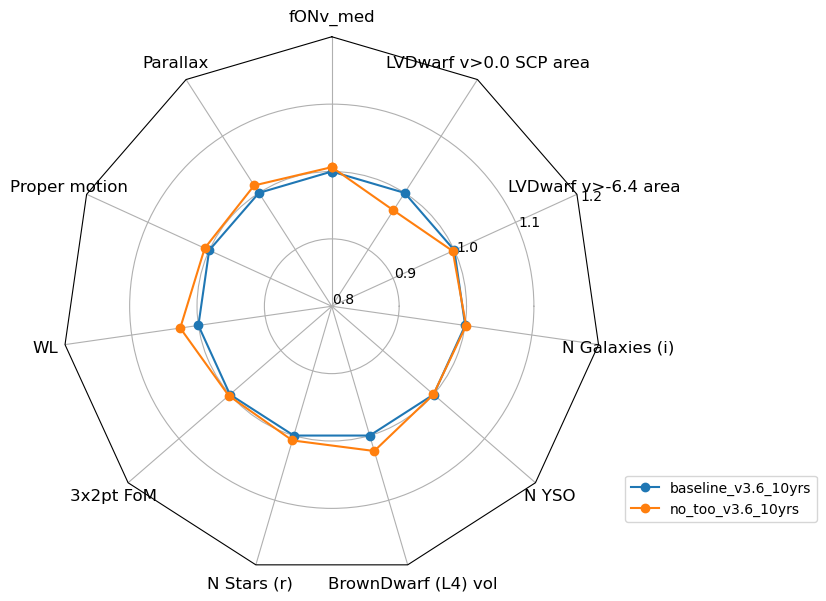
\includegraphics[width=0.5\linewidth]{figures/baseline_v36_wfd_static.png}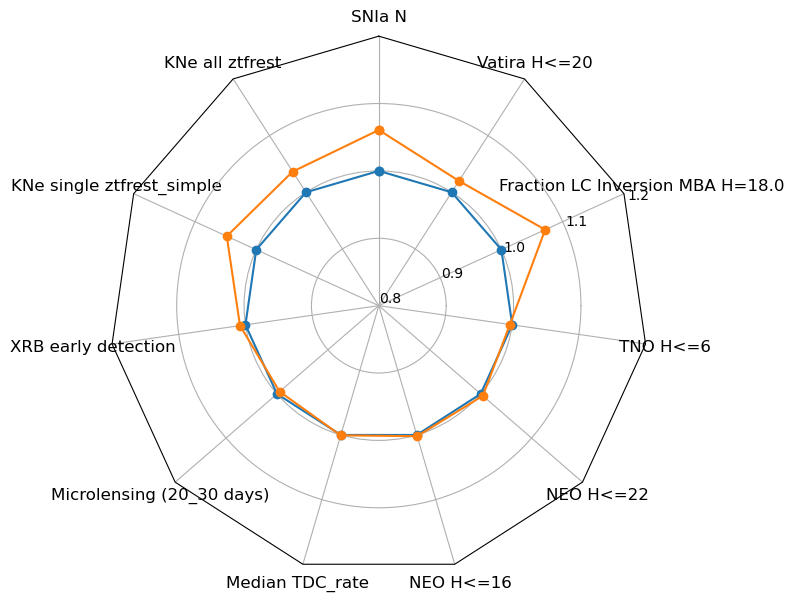
\includegraphics[width=0.5\linewidth]{figures/baseline_v36_wfd_transient.png}
    \caption{The impact of the inclusion of the ToO program on static (left) and transient and variable (right) LSST science. Note that the marginalnegative impact on the number of well-characterized SNIa (\texttt{SNIa N}) and Kilonova (KN) discovery in the WFD is compensated, respectively, by the potential for discovery of KN counterparts of MMA triggers, and by the potential of KN counterparts of gravitational waves as cosmological probes \citep{sneppen2023measuring}.}
    \label{fig:too}
\end{figure}
This report identified several different classes of ToOs for which Rubin's observations are well-justified. The vast majority of ToOs will be to follow up gravitational wave (GW) events, while a much smaller number of neutrino and solar system ToOs are expected. 

The current LIGO-Virgo-KAGRA (LVK) GW observing run (Observing Run 4 or O4) will end before the start of LSST. Hence, GW ToOs will not commence until the start of the Observing Run 5 (O5) of the LVK detectors. We note that the start time of O5 has no expected impacts on the LSST WFD or the ToO program. Improved system performance, primarily afforded by the consistent working of three detectors (with similar sensitivity), will maximize the scientific productivity of the Rubin ToO program while reducing the impact on other programs. Two working LIGO detectors at their design sensitivity, combined with a third detector working at 30-50\% that of LIGO, will reduce the skymaps to tractable sizes for rapid Rubin coverage. We encourage the LVK science collaboration and the International Gravitational Wave Network (IGWN), to prioritize a high-performing system with three working detectors over an early start of the O5 run. 

As the GW component of the ToO program takes the largest amount of time and has the most impact on WFD, to enable optimal use of Rubin resources, {\it the SCOC recommends that a meeting to follow Rubin ToO 2024 is organized closer to the start of O5 to refine the GW follow-up survey strategy with improved knowledge of the expected performance of the GW detector networks and systems in O5 and of the performance of the full Rubin system.}
%

There is no comparable time restriction for the solar system ToO program (to follow up potentially hazardous asteroids) or neutrino ToO program (to follow-up high energy neutrinos or those from a Galactic supernova). Hence, {\it the SCOC recommends that the solar system and neutrino ToOs should start as soon as possible: as soon as suitable templates are available.} 



For all ToOs, to enable ToO response from the Rubin system, a high level of automation is required. For each potential ToO, a response shall be pre-determined algorithmically, including which targets Rubin responds to and the sequence of observations, based on the transient’s characteristics. Informal systems can easily lead to mistakes. For this reason, {\it the SCOC recommends that Rubin only consider potential ToOs that emanate from vetted discovery and distribution systems that produce and dispatch fully machine-readable alerts.\footnote{At the time of writing, the SCOC understands that full automation is not currently in place for all IceCube neutrino triggers.}} The SCOC considers the current list of vetted systems to be: LIGO-Virgo-KAGRA (gravitational waves); IceCube (neutrinos); SNEWS (neutrinos); JPL Scout or Sentry for potentially hazardous asteroids. The SCOC will evaluate future systems for inclusion in this list (\eg , a new neutrino observatory) on formal request.

Human input may still be required to evaluate in real-time the value of a ToO trigger and the specific response. One (or more) Rubin members %(assigned on any given night from a group of Rubin Scientists) 
should review triggers and be allowed to, if desired, overwrite the algorithmic decision to pursue/not pursue a ToO or interrupt the ToO observing sequence. Further, to ensure that appropriate expertise is available, an Advisory Committee of community members can interact and advise the observer in real-time, with communication initiated either by the committee or by the observer. 
This Advisory Committee should be composed of community members and have a nomination-selection process (including self-nomination) to be outlined in detail before the start of survey operations, ensuring broad coverage of scientific competence and diversity along all relevant axes.
The committee, observers, and Rubin leadership will review the ToO outcomes post-factum to advise on program changes. 
{\it The SCOC recommends real-time human review of potential ToO triggers and the establishment of a Rubin ToO Advisory Committee as described above.}



\subsection{Snaps}\label{sec:snaps}
%\tbd{The SCOC awaits commissioning assessments of the viability of collecting images in a single 1x30s exposure in all filters (rather than 2x15s), which would lead to an increase in efficiency. The SCOC has thus far seen as favorable a potential switch to a single 1x30s exposure and the associated efficiency gain. If commissioning reveals that a 1x30s exposure is indeed technically viable, the SCOC should review the benefits (and potential drawbacks) of visits in a single exposure and, if adopted, reassess its recommendations in the light of this increased efficiency.}

While the LSST has originally been designed to collect two 15-second snaps for each visit, primarily to remove cosmic rays to be combined into a single visit that is subsequently processed to derive the data products, there is an opportunity to move to collect a single 30-second exposure\footnote{Note that joint with the recommendation on $u$ band exposure length and filter balance (\autoref{sec:filterbalance}) the total exposure time in all bands but $u$ drops to 29.8 seconds, and the exposure time in $u$ is 38 seconds. However, for convenience, we will continue to refer to a ``2x15 seconds'' and ``1x30 seconds'' implementation.}, as it appears that cosmic rays can be reliably rejected from a single image. The feasibility of this plan remains to be ascertained in commissioning (including from on-sky images). However, the SCOC has conducted a science-driven analysis of this proposal. 

Going from 2x15s to a single 30s brings a gain in efficiency equivalent to ~7-9\% of the survey time (associated with reduced read-time). 


Saturation limits will be slightly higher but this will only impact a small number of objects compared to the large volume of sources in the LSST universe. Other surveys are better equipped to work with those targets that are bright for LSST.
Some science cases (\eg\ Cataclysmic Variables and Flares, very fast moving solar system objects) could benefit from the separate exposures, but data products associated with the snaps would not be released individually to the public in Data Releases, only the combined image and flux difference where detected are official data products, so all those science cases would depend on pipelines contributed by the community and user-generated data products. Additionally, for these cases too, other surveys are better equipped to work within those time scales.

Thus, the SCOC does not see scientific opportunities associated with retaining the two 15s snaps that can compete with the 7-9\% gain in survey efficiency.

\emph{The SCOC recommends that, if the technical feasibility is confirmed in commissioning, the survey is conducted with single exposures. With our recommendation of modifying the exposure time for $u$ band to 38 seconds, and compensating for this extra $u$ band survey time by a short decrease in exposure across all other bands, the single visits would be 1x29.2 seconds.}

The time gained by avoiding snaps will not be allocated to any specific program in Y1 as the performance of the system is still uncertain. In the future, the SCOC will consider how the additional time may be allocated, including to special programs (\eg, microsurveys), DDFs, WFD, etc., either to compensate for unexpected performance loss or to increase science throughput.

\subsection{Deep Drilling Fields (DDF)}\label{sec:DDF}
%\tbd{The SCOC will continue working in 2023 with the community to identify the specific intra-night cadence that maximizes the science throughput of the DDF survey, while not impacting the science performed by other surveys.}

A general plan for the LSST Deep Drilling Fields (DDF) has been developed over the course of the past 15 years, starting with \cite{2009arXiv0912.0201L} through many further developments and recommendations \citep[\eg ,][]{Brandt:2018,Scolnic:2018}.
The DDF program will include
5 DDF pointings. The SCOC recommended in \citetalias{PSTN-055} that  
6-7\% of overall survey time is dedicated to the DDF program, and that each DDF receives ~20k visits
except for the COSMOS field which should receive ~40k (with accelerated coverage so that COSMOS reaches 20k visits by the end of Y3), and the 
The Euclid Deep Field South (EDFS) has a wider area equivalent to two separate pointings (sharing ~20k visits across the two pointings). However, some questions remain: 
\begin{quote}
    [\citetalias{PSTN-055}] ``\item The SCOC will continue working in 2023 with the community to identify the specific intra-night cadence that maximizes the science throughput of the DDF survey, while not impacting the science performed by other surveys.''
\end{quote}


\incomplete{The implementation of DDF intranight visits is still under development, retaining sequences of visits in multiple filters within a night, providing opportunities for fainter per-night measurements as well as sub-minute sampling for limited times. 
Tradeoffs between nightly depth, cadence, season length, and filter balance are still being explored, but the SCOC is able to make some further recommendations based on input from the SCOC DDF Task Force.}

{\it The SCOC recommends that DDF observations should be sequences of multiple WFD-like visits (as opposed to increased exposure times) to allow rapid alert generation.}
This also benefits $\sim$minute timescale science and cross-calibration of DDF and WFD observations. 

{\it The SCOC recommends that the baseline translational dithering scale of DDF observations should be reduced from 0.7 degrees to 0.2 degrees (with exploration of even smaller translational dithers compatible with instrumental signature removal and calibration needs).
}

Smaller translational dithers allow DDFs to reach increased co-added depth for static science and increased temporal coverage for time-domain sources. While larger dither is favored for low-surface brightness science, no clusters or low-surface brightness structures of interest are included in the DDF fields.


{\it The SCOC recommends that the baseline survey strategy should accommodate varying the nightly depth, filters, or cadence of different DDFs throughout the course of LSST, while maintaining the Phase 2 recommendations for the 10-year depth of each field (including the enhanced COSMOS observations to reach 10-year depth in the first 3 years).}

Adding this flexibility to DDF observations allows for periods of higher cadence necessary for some transient science (\eg , AGN or supernovae) and enables more opportunities for concentrated, contemporaneous observations with other surveys (\eg , Euclid, Roman) while maintaining the overall co-added depth for static science.

{\it The SCOC urges the Data Management and Alert Production teams to assess the feasibility of, and resources needed for, enabling nightly co-adds of sequential DDF visits and recommends that a path is developed to enable the creation of these co-adds, subtraction with deep templates, and faint alert generation (with higher latency as needed, \eg , after sunrise). 
}

Nightly co-adds are required to take advantage of the increased DDF depth in the time domain. Alerts from nightly co-adds are essential for faint time-domain sources (\eg , high-redshift AGN or supernovae). Longer timescale co-adds (\eg , weekly, monthly, yearly) and alerts should also be considered.





\FloatBarrier

\subsection{Early Science}\label{sec:early}
% \tbd{The SCOC recommends implementing a detailed coordination plan with the Early Science Rubin team to reach a final recommendation on the strategy to be implemented in the first year of the survey, including a scheme for the construction of templates.}

 The SCOC emphasizes that the priority in Y1 of operations should be obtaining a dataset that supports and facilitates science throughout the survey. This includes a dataset sufficient for calibration across the $\sim 20,000$ square degrees of the WFD, including images at different airmasses, illuminations, field crowdedness etc. 
 
 The SCOC supports Rubin's commitment to acquiring incremental templates throughout Y1 to begin dispatching alerts (via the Alert Brokers) and encourages the Observatory to release alerts as early as possible. The SCOC reviewed the Alert Production team proposal to prioritize timeliness over the quality of templates and build templates from fewer images ($\geq 3$) in Y1 than in subsequent years. Releasing some alerts in Y1 is an important goal to enable the time domain science community to prepare for the full-volume full-fidelity alert streams to come in subsequent years, as well as increasing the discovery potential of LSST in early operations. However, this goal should not overwrite the priority of obtaining a fully calibrated system by the end of Y1.

 The SCOC recommends that the filter balance is slightly modified in Y1 to acquire a sufficient number of $u$ band images for calibration. 

 The SCOC does not recommend beginning rolling before the end of Y1. In the months following the release of this recommendation, the SCOC will continue to work on the implementation of rolling (\autoref{sec:rolling}) to better understand its interplay with potential Y1 outcomes. 

%\subsection{Euclid}\label{sec:Euclid}
%\tbd{The SCOC shall work in coordination not only with the scientific community but also with the leadership of Rubin and the Euclid mission to identify cadence requirements, co-observing strategies, and paths to produce the data products that will enhance science through the coordinated observing of the EDFS.}

\FloatBarrier



